\documentclass[11pt]{article}
%%%%%%%%%%%%%%%%%%%%%%%%%%%%%%%%%%%%%%%%
\usepackage{amsmath}
\usepackage{verbatim}
\usepackage[usenames,dvipsnames]{color}
\usepackage{setspace}
\usepackage{lscape}
\usepackage{longtable}
\usepackage[top=1.25in,bottom=1.25in,left=1in,right=1in]{geometry}
\usepackage{graphicx}
\usepackage{epstopdf}
\usepackage[usenames,dvipsnames]{pstricks}
\usepackage{epsfig}
\usepackage{pstricks-add}
\usepackage{pst-node}
\usepackage{pst-plot}
\usepackage{fancyhdr}
\usepackage[absolute,showboxes]{textpos}
\usepackage{booktabs}
\usepackage{dcolumn}
\usepackage{arydshln}
\usepackage{natbib}
\usepackage{tabularx}
\usepackage{subfigure}

\setcounter{MaxMatrixCols}{10}
\newcolumntype{d}[1]{D{.}{.}{-2.#1}}
\newenvironment{proof}[1][Proof]{\noindent\textbf{#1.} }{\ \rule{0.5em}{0.5em}}
\setlength{\columnsep}{.2in}
\psset{unit=1cm}

\def\sym#1{\ifmmode^{#1}\else\(^{#1}\)\fi}

\begin{document}
\begin{titlepage}
\vspace{2in} \noindent {\large \today}

\vspace{.5in} \noindent {\Large \textbf{\strut How Tight are Malthusian Constraints?}}

\vspace{.25in} \noindent {\large T. Ryan Johnson}

\vspace{.05in} \noindent University of Houston

\vspace{.25in} \noindent {\large Dietrich Vollrath}

\vspace{.05in} \noindent University of Houston

\vfill \noindent \textsc{Abstract} \hrulefill

\vspace{.05in} \noindent The Malthusian constraint of using land in agricultural production is central to theories of stagnation and the take-off to growth, as well as in studies of contemporary developing countries. The elasticity of agricultural output with respect to land captures this constraint, and we provide a methodology to estimate this elasticity using variation in rural densities across different locations. We use district-level data from around the globe on rural densities and inherent agricultural productivity to estimate the elasticity for various sub-samples. We find the Malthusian constraint it tightest (i.e. the elasticity is highest) in temperate areas such as Europe, parts of North America, northern China, and North Africa. The constraint is loosest in tropical and sub-tropical areas such as Southeast Asia, Central America, and central Africa. We discuss how tighter Malthusian constraints result in greater sensitivity of non-agricultural employment, real wages, and population dynamics to shocks in population size and technology, with implications for the study of both historical economies and developing nations today.

\vspace{.1in} \hrule

\vspace{.5in} \noindent {\small JEL Codes: O1, O13, O44, Q10}

\vspace{.1in} \noindent {\small Keywords: land constraints, Malthusian stagnation, agriculture}

\vspace{.1in} \noindent {\small Contact information: 201C McElhinney Hall, U. of Houston, Houston, TX 77204, devollrath@uh.edu. We thank seminar participants at the London School of Economics for their comments. All errors remain our own.}
\end{titlepage}

\pagebreak 

\section{Introduction}
\onehalfspacing 
A common assumption in studying historical or contemporary development is that a finite (or inelastic) resource, namely agricultural land, is necessary for production. We refer to this as a ``Malthusian constraint'', and \textit{ceteris paribus}, this constraint implies that living standards are declining with the absolute size of the population. Combining the Malthusian constraint with a positive relationship of living standards and population growth yields the canonical Malthusian model of stagnation \citep{ashraf2010dynamics}, and forms the basis for models of the transition from stagnation to sustained growth.\footnote{The literature on the transition has grown large enough that it is difficult to provide a reasonable overview in a footnote. An overview of this unified growth literature can be found in \citet{Galor:2011uq}, who cites several key contributions \citep{gw00,galor2002natural,Hansen:2002fk,doepke2004accounting,cs2005,lagerlof2006,craftsmills2009,strulik2008population}. Explanations for the Great Divergence in income per capita are often framed in terms of these unified growth models \citep{kp2001,galor2008trading,vollrath2011,vv08,vv13,cs2015}.} The Malthusian constraint features in quantitative work on contemporary developing countries that rely on agriculture \citep{Gollin:2007oq,Restuccia:2008hc,weilwilde2009,Gollin:2010ys,ev2016clim,ev2016}, and is even relevant for long-run growth in relatively rich countries due to possible limits to resources \citep{perettovalente2015}.

The ``tightness'' of this Malthusian constraint is determined by the elasticity of agricultural output with respect to agricultural land. This elasticity, in turn, dictates the sensitivity of living standards (i.e. the average product of labor) to the size of the population. A ``tight'' Malthusian constraint occurs when the elasticity is large, and living standards are very sensitive to the size of the population. In contrast, a ``loose'' Malthusian constraint occurs when the elasticity is small, and living standards are insensitive to population size. Knowing the elasticity of agricultural output with respect to land lets us quantify the effects of population or productivity changes on living standards. Moreover, if there is \textit{variation} in this elasticity across economies, it tells us that Malthusian constraints may have been more or less binding on their development.

In this paper we propose a methodology to estimate the elasticity of agricultural output with respect to land, and thus quantify the tightness of the Malthusian constraint. To derive an empirical specification for estimating the elasticity, we develop a model of production with agricultural land that expands on the standard one-sector version. First, we consider an economy that is made up of many locations, each with its own stock of agricultural land, but where labor and other inputs move freely between those locations. This reveals a simple cross-sectional relationship between the density of agricultural workers in a location and agricultural total factor productivity (TFP), and we can recover a direct estimate of the elasticity from this relationship. Second, we allow for the presence of factors beyond just land and labor, showing that our estimation strategy does not rely on data on these other inputs. Third, we allow for a non-agricultural sector that employs labor. This shows that the spatial relationship of \textit{agricultural} workers and agricultural TFP holds regardless of the aggregate level of agricultural employment or overall development. The spatial distribution of agricultural workers across districts \textit{within} provinces or states is informative about the elasticity of agricultural output with respect to land. We can leverage data from countries at all levels of development, historic or contemporary, to estimate the elasticity. Further, by looking at districts \textit{within} provinces or states to make our estimates, we do not need to rely on cross-country comparisons.

We assemble our data at the district level (i.e. 2nd level administrative units within countries) for rural population density in the year 2000 from \citet{hyde31}, and combine that with an measure of the caloric yield of districts built on the data from \citet{galorozak2016} to capture an exogenous measure of inherent agricultural TFP. As in their work, our measure is built on agro-climatic constraints plausibly unaffected by human activity (e.g. soil quality and length of growing season) from \citet{gaez}, combined with information on the calorie content of various crops. We explain in more detail below, but our measure of the caloric yield within a district deviates slightly from Galor and {\"O}zak's methodology, in that we evalute the calorie-maximizing crop choice for each grid cell within a district, and aggregate up to an overall caloric yield, rather than averaging the caloric yield across all crops.

In the end, we have a dataset of 32,862 districts, coming from 2,471 provinces in 154 countries. Using this data, we provide estimates of the elasticity of agricultural output with respect to land. Further, we find that there is substantial variation in this Malthusian constraint across regions of the world. The variation is closely related to climate zones and dominant crop types. Specifically, tropical areas that are suitable for crops such as rice, maize, and millet have much lower elasticities than temperate areas suitable for crops such as oats, rye, and wheat. Among the tightest constraints are those in Europe (estimated elasticity of 0.274), the U.S. and Canada (0.190), and Northern Africa (0.281). In comparison, South and Southeast Asia (0.160), tropical Africa (0.097), and the tropical Americas (0.125) have the loosest land constraints. Within China, the temperate areas have among the tightest constraints estimated (0.522), while the sub-tropical areas of China have a loose constraint (0.118), just below that found for Japan (0.178) and the Koreas (0.214). 

This variation appears to be related to climate type. We estimate effects after dividing districts by their climate characteristics and find that equatorial areas, and those with dry winters and/or monsoonal precipitation, tend to have loose land constraints, while temperate and cold areas, and those with regular year-round rainfall, tend to have tight constraints. This holds as well when dividing districts based on their suitability for various crops, which is tied to climate characteristics (as well as features such as soil quality). We find that the elasticity is consistently low (around 0.150) when we look only at districts that are capable of growing crops such as cassava, pearl millet, yams, and paddy rice. In contrast, the elasticity is larger when examining provinces that are able to raise crops such as oats, rye, wheat, and (white) potatoes (elasticities of around 0.222). Note that these findings are based on within-country comparisons, meaning that rice-growing areas of specific countries demonstrate lower elasticities than wheat-growing areas within those same countries.

The estimated size of the elasticities, and their patterns across regions and climate types is robust across a variety of specifications. All regressions include controls for the percent of a district that is urban, as well as the density of nighttime lights, as a proxy for the level of development. The results hold using rural population data from 1950 or 1900 from \cite{hyde31}, and also if estimated using province-level variation in rural density and productivity with country fixed effects. We use alternative measures of the land area, finding similar results, and discuss how measurement error in this variable is unlikely to be driving our results. Finally, our baseline specification is built on several assumptions regarding the mobility of factors and output across districts. Changing those assumptions suggests different specifications with alternate control variables, but these deliver similar results in terms of the estimated elasticity of agricultural output with respect to land.

Our approach to estimating this elasticity has several advantages compared to the existing literature. The standard approach has been to use country-level panel data \citep{Hayami:1970ly,Hayami:1985cr,cpr1997,mm2001,Mundlak:2000dq,mbl2012,et2013mango} to estimate agricultural production functions, with a common set of coefficients across countries for each input, including land. Issues here are with unobserved productivity, the heterogeneity of coefficients, and the measurement of non-land inputs. Some have examined heterogeneity \citep{gg2003,Wiebe2003Resource-Qualit}, while others have attempted to estimate heterogenous coefficients using factor analysis to address unobserved productivity \citep{et2013mango,ev2016clim,ev2016}. Relative to this work, our paper uses a direct measure of inherent productivity, while our district-level data allows us to control for unobserved country and province-level effects. As shown below, our specifications do not need any data on non-land inputs, avoiding measurement error of those, or even the need to define them precisely. The district-level data also allows us to examine heterogeneity in the estimated elasticity for land at a much finer level than prior work, including heterogeneity within country. 

The heterogeneity we identify in the Malthusian constraint across regions and climate types has implications for several questions in historical and contemporary development. Expanding on the model we used to drive the empirical work, we show that the tighter the Malthusian constraint, the more sensitive the agricultural labor allocation and real wage are to population and technological shocks. Thus temperate areas, with relatively cool summers and regular rain, like much of Europe and North America, will be more influenced (for better or worse) by changes in population or technology.

This may help explain why the Black Death appeared to have been such a significant shock to European development, while similar epidemics in Asia had more muted effects \citep{McNeill1976}. With a tight land constraint in Europe, the drop in population from the Black Death would generated a much larger drop in the agricultural labor share, and a much larger increase in the real wage, than in Asia. These effects may have been sufficient to push Europe into a new equilibria with respect to urban mortality and/or demographic behavior \citep{vv13,vv08}. 

The process of ``involution'' \citep{Geertz1963,Huang1990}, and why it was associated with South-east Asia and China, may be associated with the loose Malthusian constraint in these areas. Involution involves an intensification of agriculture, in the sense of increased density of workers per hectare, but without involving gains in living standards. Due to the loose land constraint, technological improvements would have had small effects on real wages, translating instead into increased density. Hence South-east Asia and China would appear to experience involution compared to Europe, even if they were experiencing similar growth in productivity.

Beyond the historical setting, Malthusian constraints may have relevance for contemporary developing economies. Quantitatively, \citet{ev2016clim,ev2016} establish that differences in the elasticities of the agricultural production function, including the land elasticity, change the growth prospects of heavily agricultural countries. They find that countries in regions with loose land constraints may need to experience growth in agricultural productivity and input use (e.g. fertilizers and capital) five to ten times higher than areas with tight land constraints, just to hit similar targets for the agricultural labor share and agricultural output per capita.

More broadly, our work is related to several recent studies on the the role of geography and/or inherent agricultural productivity in development \citep{oh2005,ashraf2010dynamics,Nunn2011,Nunn2012,mich2012,agn2013,cook2014role,cook14,fenske2014,alsan2015,ashrafmich2015,dks2015,galorozak2016,litina2016,ads2016,FrankemaPap2017}. Unlike those papers, ours does not propose a direct causal relationship between geography and development, but rather suggests that any proposed causal impact may have differential effects based on the size of the Malthusian constraint. By itself the size of the constraint does not dictate whether a country is rich or poor, but translates changes in productivity and population into changes the agricultural labor share, real wage, and distribution of population across locations.

There are two studies that share a focus on the distribution of labor and economic activity. The first is \citet{mfm2014}. Those authors examine the growth of urbanization at the grid-cell level, specifically the timing of when grid-cells pass certain thresholds of urban population density (i.e. 5.67 urban residents per square kilometer, equivalent to 5,000 urban residents in a grid cell near the poles), or the percent of urban population in the cell. They estimate a homogenous relationship, while we focus on heterogeneity in the relationship of (rural) population density and agricultural productivity, and use the more nuanced measure of agricultural caloric productivity than the index from \citet{ramankutty2002} that they rely on. The second related study is \citet{hssw2016}, who examine the spatial distribution of economic activity (closely associated with urbanization) at the grid-cell level using night lights, relating it to geographic characteristics associated with either agriculture or trade. While our work uses the geographic distribution of rural population to estimate Malthusian land constraints, it has no implications for the spatial distribution of \textit{urban} activity, and our results are entirely complementary with theirs.

To continue, we first use a simple model and cross-country data to define the land constraint and illustrate how we estimate it. Following that, we derive a relationship of rural density and agricultural productivity that incorporates non-labor inputs as well as a fixed factor of production, allows for multiple locations, and incorporates a non-agricultural sector. Using the relationship developed in the model, we then turn to estimating the Malthusian land constraint. We describe the data we use, and perform the estimations on different sub-samples distinguished by regions, crop suitability, and climate zones. Given those results, we then discuss the implications of the heterogeneity in land constraints for explaining development, and the final section of the paper concludes.

\section{A Simple Model and Simple Data}
To set ideas, we start with a simple one-sector model of production involving a fixed factor of production and labor only. We use this to describe the Malthusian land constraint, and show how the level of population density does not provide any information on the constraint. Following that, we illustrate differences in the land constraint across major regions using data from 1500CE. 

\subsection{Density and the Malthusian Constraint}
Consider an economy with a simple production function that uses land ($X$) and labor ($L$) in production, as in a typical Malthusian model,
\begin{equation}
Y = A X^\beta L^{1-\beta}.
\end{equation}
$A$ here is total factor productivity. If we solve for the average product of labor, we have
\begin{equation}
    \frac{Y}{L} = A \left(\frac{X}{L}\right)^{\beta}.
\end{equation}

The ``tightness'' of the land constraint is captured by $\beta$. In this simple model, this is both the elasticity of output with respect to land, but also the elasticity of the average product of labor with respect to the amount of labor, $L$. $\beta$ tells us how strong of an effect changes in population will have on the living standards, which would form a key relationship in any Malthusian model.

When $\beta$ goes to one, land becomes the only factor relevant to production. In this case, the average product of labor ($Y/L$) becomes very sensitive to the size of $L$ as well, with an elasticity of negative one. A high value of $\beta$ thus implies a ``tight'' Malthusian constraint. On the other hand, as $\beta$ goes to zero, land becomes irrelevant to production, and the land constraint is ``loose''. In this case, the average product labor is insensitive to $L$, with an elasticity of zero.

Note that it is not TFP, $A$, that dictates whether the land constraint is tight or loose. We could have an economy with a very high level of agricultural productivity but with a tight constraint because $\beta$ is large. And it is possible to think of economies with low productivity ($A$ is low), but with a loose Malthusian constraint because $\beta$ is relatively small.

The simple model also allows us to show why population density itself is not useful in determining the tightness of the land constraint. Assume that there is some population process such that output per person is stagnant at the level of $c$. In this case, then population density will be
\begin{equation}
    \frac{L}{X} = \left(\frac{A}{c}\right)^{1/\beta}.
\end{equation}
The level of density depends on the size of $A$ relative to $c$, and $\beta$ does not tell us whether $A/c$ is big or small. We cannot infer how \textit{sensitive} population density is to productivity (i.e $1/\beta$) from the \textit{level} of population density. The ambiguity of population density shows up when comparing the use of this metric across different sources. \citet{pom2000} suggests that both Europe and China faced similar ``Malthusian pressures'', despite the lower population density in Europe. Others \citep{Elvin1973,huang2002} point to the high density in China as evidence of Malthusian constraints binding more tightly than in Europe. In a contemporary setting, \citet{conleyetal2007} claim Africa is in the midst of a Malthusian crisis, despite being one of the most sparsely populated areas on the planet. 

As the simple model makes clear, the Malthusian constraint can not be inferred from the \textit{level} of density, but rather from \textit{changes} in density. Before turning to some suggestive data, note that if we take logs of the above equation,
\begin{equation}
	\ln L/X = \frac{1}{\beta} \ln A - \frac{1}{\beta} \ln c, \label{EQ_LX}
\end{equation}
we recover a linear relationship between (log) density and (log) productivity. The slope of this relationship is $1/\beta$, and so examining data on density and productivity should allow us to infer the tightness of the Malthusian constraint.

\subsection{Evidence on Density and Productivity, 1500CE}
\citet{ashraf2010dynamics} provided systematic evidence consistent with the basic predictions of a Malthusian model of population and production. Their data was at the country level, and their baseline results include simple linear regressions showing a positive relationship of population density in 1500 C.E. (as well as in 1000 C.E. and 1 C.E) with both the number of years since the Neolithic agricultural revolution and a measure of agricultural productivity. This productivity measure is based on a suitability measure from \citet{ramankutty2002} and a measure of the percent of land that is arable in a country. These are combined using principal components to arrive at a single index of agricultural productivity, which is based only on agro-climatic characteristics.

Referring back to the theoretical work above, equation (\ref{EQ_LX}) indicates that the elasticity of population density with respect to productivity should reflect (inversely) the tightness of the Malthusian constraint. Do we see variation in this elasticity, and hence variation in the tightness, across major regions of the world?

To answer this, we divided the original Ashraf/Galor sample into regional groups: Europe, Asia, Middle East and North Africa, Sub-Saharan Africa, and the Americas.\footnote{In defining which countries belong to which regions, we deviate slightly from those authors. Russia was excluded from all regions, as it does not clearly fall into any single one. Several countries are in both our Middle East and North Africa region, as well as in the Asia region. Nothing about this cross-country analysis depends on that definition. Sub-Saharan Africa is, as expected, Africa less the traditionally Islamic North African nations.} We then replicated the Ashraf and Galor analysis for each region separately.

The results are best seen in Figure \ref{FIG_ag_regions}, which plots log population density in 1500 CE against the residual measure of agricultural productivity after we controlled for the additional regressors used by Ashraf and Galor in their analysis.\footnote{The specific controls are (log) years since the Neolithic transition, (log) absolute latitude, the mean distance to a coast or river, and the percent of land less than 100 km from a coast or river. Continent dummies were not included as they are colinear with our regions.} The residual for agricultural productivity from these regressions are what is plotted on the x-axis in Figure \ref{FIG_ag_regions}. By plotting the actual log population density in 1500 CE on the y-axis, one can still see the distinct level differences in density across these regions.

What becomes immediately apparent from Figure \ref{FIG_ag_regions} is that Europe is an outlier in several respects. Note that population density has a zero slope with respect to residual productivity, implying that $\beta$ is very \textit{large}, and hence the Malthusian constraint is very \textit{tight}. Places within Europe that are more productive are not more dense, which contrasts with the three other regions plotted in the figure. Asia, the Mideast and North Africa, and Sub-Saharan Africa conform to the original results in Ashraf and Galor, while Europe does not. Given the positive slopes in these regions, the implied value of $\beta$ is low relative to Europe, indicating looser land constraints.

Given that we are looking at sub-samples of a cross-country dataset, and given that the residual variation in productivity within Europe is noticably smaller than in other regions, we do not want to overstate the results in Figure \ref{FIG_ag_regions}. In the following sections we will verify these results by looking at within-country data, and find that similar patterns show up.

\section{Productivity, Rural Density, and the Malthusian Constraint}
To move towards estimations that should be more reliable, we develop an extended version of the simple model we started with. This extended model shows us that we can use variation in agricultural worker's density across locations to infer the size of the Malthusian constraint. That model incorporates multiple locations, non-labor inputs aside from the fixed factor, and a non-agricultural sector, and thus shows us how to handle those elements in our empirical work.

\subsection{Agricultural Production Across Locations}
Consider a region (e.g. province or state) $I$ that contains a set of districts, each denoted by $i$. The aggregate agricultural production function for district $i$ is given by 
\begin{equation}
Y_{i} = A_{i} X_{i}^{\beta} \left(K_{Ai}^{\alpha}L_{Ai}^{1-\alpha}\right)^{1-\beta} \label{EQ_production}
\end{equation}
where $A_{i}$ is total factor productivity, $X_{i}$ is land, $K_{Ai}$ is capital (or any other inputs aside from land and labor), and $L_{Ai}$ is the number of agricultural workers. The tightness of the Malthusian land constraint is captured by $\beta$. Note that we presume $\beta$ is not specific to the distict $i$, but rather common to the region $I$ in which this district lies.

Consider the average product of labor in this district, which is
\begin{equation}
	\frac{Y_i}{L_{Ai}} = \frac{A_{i} X_{i}^{\beta} K_{Ai}^{\alpha(1-\beta)}}{L_{Ai}^{\alpha + \beta(1-\alpha)}}.
\end{equation}
Writing is this way makes clear that the elasticity of the average product with respect to $L_{Ai}$ is $\alpha + \beta(1-\alpha)$, holding $X_i$ and $K_{Ai}$ constant. As in the simple model, this is increasing in $\beta$, although no longer equal to $\beta$.  If we hold the capital/labor ratio, $K_{Ai}/L_{Ai}$, constant then the elasticity of the average product with respect to $L_{Ai}$ is again equal to $\beta$. The tighter is the land constraint, $\beta$, the more sensitive is the average product of labor to the amount of labor employed.

The amount of labor employed in district $i$ will depend on its productivity relative to other districts in the same region. We assume that both labor and capital are mobile across districts within region $I$, and hence the wage, $w$, and return on capital, $r$, are the same for each district $i$. In each district those wages and returns are determined by the following equations
\begin{eqnarray}
    w = \phi_L \frac{Y_i}{L_i} \\ \nonumber
    r = \phi_K \frac{Y_i}{K_i} \label{EQ_factorprices}
\end{eqnarray}
where $\phi_L$ and $\phi_K$ are the fraction of output paid to labor and capital, respectively. These fractions may or may not be equal to the respective elasticities in the production function of these inputs, meaning that the wage and rate of return may or may not be equal to the marginal product of these factors. We set the model up this way to make two things clear. First, that we are not going to identify the value of $\beta$ by using information on shares of output, and second that our empirical work only depends on these factors being mobile across districts, not on them being paid exactly their marginal product.

Given that all districts face the same wage and rate of return, in each district the capital/labor ratio will be the same at
\begin{equation}
    \frac{K_i}{L_{Ai}} = \frac{w}{r}\frac{\phi_K}{\phi_L}.
\end{equation}
Using this ratio, we can write production in each district $i$ as
\begin{equation}
Y_{i} = A_{i} X_{i}^{\beta} \left(\frac{w}{r}\frac{\phi_K}{\phi_L}\right)^{\alpha(1-\beta)} L_{Ai}^{1-\beta} \label{EQ_prodwr}
\end{equation}
which relates production in district $i$ to district level productivity, $A_i$, land, $X_i$, and labor, $L_{Ai}$, but also the \textit{region}-specific $w/r$ ratio.

Combine the wage definition from (\ref{EQ_factorprices}) and the production function in (\ref{EQ_prodwr}) with an adding-up condition for agricultural labor 
\begin{equation}
\sum_{i\in I} L_{Ai} = L_A,
\end{equation}
where $L_A$ is the total amount of agricultural labor in region $I$. These can be solved for the density of agricultural workers in sub-unit $i$,
\begin{equation}
\frac{L_{Ai}}{X_i} = A_{i}^{1/\beta}\frac{L_A}{\sum_{j\in I} A_{j}^{1/\beta}X_{j}}. \label{EQ_LaX}
\end{equation}
Intuitively, any district that is particularly productive should have a greater share of the agricultural labor force employed in it. In addition, the larger is the region-wide agricultural labor force, $L_A$, the more dense is agricultural labor in any given district.

Note that the fraction on the right is common to every district in the region. Take logs of (\ref{EQ_LaX}) 
\begin{equation}
\ln L_{Ai}/X_i = \frac{1}{\beta} \ln A_{i} + \ln \Gamma, \label{EQ_est}
\end{equation}
where
\begin{equation}
    \Gamma = \frac{L_A}{\sum_{j\in I} A_{j}^{1/\beta}X_{j}}.
\end{equation}
This equation shows that the elasticity of agricultural population density with respect to the level of produtivity is $1/\beta$, and is thus captures the (inverse of) the tightness of the Malthusian constraint. A version of the linear expression in (\ref{EQ_est}) is what we will take to the data in the empirical section. Note that $\Gamma$ is common to all districts within the region, and is not $i$-specific. We will thus be able to use fixed effects to capture this term, and we do not need to know the economics of how $L_A$ is set in order to recover estimates of $\beta$. Our approach does not us require any sort of assumptions about how the demand for agricultural goods is determined (which would dictate the region-wide level of $L_A$).

If we observe agricultutral labor spread evenly across districts regardless of their productivity ($1/\beta$ approaches zero), then this implies a tight Malthusian constraint. Agricultural workers cannot crowd into the highest productivity district because this would drive down their average product. On the other hand, observing agricultural labor concentrated into the most highly productive districts ($1/\beta$ is large) will imply that Malthusian constraints are loose. Workers are able to crowd into the productive districts as this would have little effect on their average product.

\subsection{Non-agricultural Employment and Real Income}\label{SEC_LAL_y}
As noted, we do not have to specify how $L_A$ is determined at the province level in order to make our estimates of $\beta$. But to show the \textit{effect} of $\beta$ on outcomes like the province level share of labor in agriculture, $L_A/L$, or a measure of real wages, we need to add more structure to the model.

Total agricultural supply in province $I$ can be written as
\begin{equation}
Y_A = \sum_{i \in I} A_{i} X_{i}^{\beta} \left(K_{Ai}^{\alpha}L_{Ai}^{1-\alpha}\right)^{1-\beta}, \label{EQ_caL}
\end{equation}
where each district $i$ has a production function matching equation (\ref{EQ_production}). We know each $L_{Ai}$ from (\ref{EQ_LaX}). By a similar logic we can establish that the allocation of capital to any individual location $i$ is
\begin{equation}
	K_{Ai} = A_{i}^{1/\beta} X_i \frac{K_A}{\sum_{j\in I} A_{j}^{1/\beta}X_{j}} \label{EQ_KaX}
\end{equation}
where $K_A$ is the aggregate allocation of capital to agriculture. Combine (\ref{EQ_LaX}) and (\ref{EQ_KaX}) with the expression in (\ref{EQ_caL}) and we can solve for 
\begin{equation}
	Y_A = A_A \left(\frac{K_A}{L_A}\right)^{\alpha(1-\beta)} L_A^{1-\beta}, \label{EQ_caL_solve}
\end{equation}
where 
\begin{equation}
    A_A = \left(\sum_{j\in I} A_{j}^{1/\beta}X_{j} \right)^\beta
\end{equation}
is the measure of aggregate agricultural total factor productivity for the province.

For non-agriculture, we specify province level production as 
\begin{equation}
    Y_N = A_N \left(\frac{K_N}{L_N}\right)^{\alpha} L_N. \label{EQ_YN}
\end{equation}
We could write out district-specific functions and solve for allocations similar to what we did for agriculture. But that is not necessary for our analysis.

For preferences, we follow \cite{boppart2014}, who specifies a functional form for the indirect utility function that allows for analysis of structural change that involves income effects.\footnote{The functional form is a form of ``price independent generalized linearity'' (PIGL) preferences}. This function has non-linear Engel curves while still allowing for aggregation across individuals, and results in a simple demand function for agricultural goods ($c_A$), in log form, of
\begin{equation}
    \ln c_A = \ln \theta_A + (1-\epsilon) \ln M + (\gamma - 1) \ln p_A + (\epsilon - \gamma) \ln p_N \label{EQ_ca_demand}
\end{equation}
where $\theta_A$ is a preference parameter, $M$ is nominal income, and $p_A$ and $p_N$ are the prices of agricultural and non-agricultural goods, respectively. With $0 < \epsilon < 1$, these preferences imply that the income elasticity of agricultural demand is less than one. Further, assuming $\epsilon > \gamma$ means individuals are willing to subsitute between agricultural and non-agricultural goods in response to relative prices.\footnote{The relative size of $\epsilon$ and $\gamma$ is the opposite of what Boppart uses to describe the shift from manufacturing to services, where an increasing expenditure share on services is accompanied by \textit{higher} prices in that sector, indicating complements. Here, the expenditure share of non-agriculture rises while also having \textit{lower} prices.}

To go further, we specify the shares of output paid to capital, land, and labor in each sector. The most important assumption we make is that the share of output paid to land in the agricultural sector is zero, equivalent to assuming zero property rights over land. This does not impact the effect of $\beta$ acting through the curvature of the production function, but does eliminate the effect of $\beta$ acting through factor shares. With the land share set to zero, we assume that the share paid to capital in both sectors is $\phi_K$, and to labor, $\phi_L$. It is not essential for those shares to equal $\alpha$ and $(1-\alpha)$ for our results.

With these shares, it follows that the capital/labor ratio in both sectors is equal to the aggregate capital labor ratio,
\begin{equation}
    \frac{K_A}{L_A} = \frac{K_N}{L_N} = \frac{K}{L} = \frac{w}{r}\frac{\phi_K}{\phi_L}.
\end{equation}
Further, with labor mobile between agriculture and non-agriculture, the value marginal product of labor must be equal across sectors, so that
\begin{equation}
    p_A \phi_L \frac{Y_A}{L_A} = p_N \phi_L \frac{Y_N}{L_N}. \label{EQ_mobility}
\end{equation}
Combining the production functions in (\ref{EQ_caL_solve}) and (\ref{EQ_YN}), the demand function in (\ref{EQ_ca_demand}), the equilibrium condition in (\ref{EQ_mobility}), and conditions that supply equals demand ($Y_A = c_A L$ and $Y_N = c_N L$) we can solve for the share of labor employed in agriculture (see the appendix for details on the algebra). In log terms,
\begin{equation}
    \ln L_A/L = \ln \theta_A + \frac{\beta\gamma}{1-\beta\gamma} \ln L - \frac{\gamma}{1-\beta\gamma} \ln A_A + \frac{\gamma - \epsilon}{1-\beta\gamma} \ln A_N + \frac{\alpha(\beta\gamma - \epsilon)}{1-\beta\gamma} \ln K/L. \label{EQ_lnLAL}
\end{equation}
From this, the elasticities of the agricultural labor share with respect to productivity ($A_A$ and $A_N$) and population ($L$) are easily seen. In each case, note that the elasticity is \textit{increasing} with the size of $\beta$.

We can solve for real income as well. In terms of agricultural goods, real income is $y = M/p_A$, similar to a ``grain wage'' in the terminology used in studies of historical living standards \citep{allen2005,bg2006,allen11}. Again relegating the algebra to the appendix, we can solve for real income ($y$) as
\begin{equation}
    \ln y = \frac{1}{1-\beta\gamma} \ln A_A - \frac{\beta}{1-\beta\gamma} \ln L + \frac{\beta(\epsilon-\gamma)}{1-\beta\gamma} \ln A_N + \frac{\alpha(1-\beta) + \alpha\beta(\epsilon-\gamma)}{1-\beta\gamma} \ln K/L. \label{EQ_lny}
\end{equation}
The elasticities with respect to productivity ($A_A$ and $A_N$) and population ($L$) are easy to pick out from this expression. As with the labor share, the elasticities are all increasing in $\beta$. The combination of (\ref{EQ_lnLAL}) and (\ref{EQ_lny}) show the importance of the size of Malthusian constraints for development. Technological or population shocks will have more severe effects, either positive or negative, on locations that have tighter Malthusian constraints. 

The larger is $\beta$, the more sensitive is the average product of agricultural workers to the number of workers in that sector. This means that in response to any shock that pushes people \textit{into} agriculture, the average product falls very quickly, which creates an incentive for more workers to enter that sector to meet demand for agricultural goods. To make that happen, the relative price of agriculture has to rise, and the number of workers in non-agriculture falls by a lot, meaning living standards fall. In contrast, for any shock that pushes people \textit{out} of agriculture, the average product of the remaining workers rises very quickly, which allows even more workers to leave agriculture. For that to happen, the relative price of agriculture has to fall, and as the number of workers in non-agriculture rises, so does real income.

If Malthusian constraints are loose, and $\beta$ is small, there is little effect of the movement of workers on the average product of agricultural workers. Thus in response to shocks (in either direction), there is little change in the average product of labor, and hence little incentive for more workers to move into or out of agriculture. Thus the shifts in labor share, $L_A/L$, and real income, $y$, are more muted when $\beta$ is smaller.

When we consider steady improvments in technology ($A_A$ and/or $A_N$) over time, locations with tight Malthusian constraints will see a more rapid transition away from agriculture, and more rapid growth in real incomes, than locations with loose Malthusian constraints. But note that this does not imply that places with tight constraints are necessarily richer. The level of $A_A$ and $A_N$ are determined exogenously in this model, and there is nothing that forces those technology terms to be higher (or lower) in locations with high $\beta$. Nevertheless, the size of the Malthusian constraint plays an important role in determining how economies respond to technological and population growth. 

\section{District level estimates}
We move to sub-national data on rural population density and agricultural productivity, and demonstrate that there are differences in Malthusian land constraints across different regions and climate types. The basis of our estimations is equation (\ref{EQ_est}). We rewrite that here as a regression specification,
\begin{equation}
	\ln A_{isc} = \alpha + \beta \ln L_{Aisc}/X_{isc} + \gamma_{sc} + \delta' \mathbf{Z}_{isc} + \epsilon_{isc}. \label{EQ_regress}
\end{equation}
On the left is agricultural productivity in district/prefecture/county $i$ (e.g. Shaoguan) of province/state $s$ (e.g. Guangdong) in country $c$ (e.g. China). This is regressed on \textit{agricultural} population density. We elided the distinction regarding agricultural population in the prior section on cross-country data, but it is crucial to note that it is the relationship of agricultural workers to productivity that informs us about the tightness of the Malthusian constraint.

As is obvious, we have rearranged the relationship to have agricultural productivity as the \textit{dependent} variable, and regress that on agricultural population density. This allows us to recover an estimate of $\beta$ directly. Leaving the regression equation as in (\ref{EQ_est}), we would be estimating $1/\beta$, and as an inverse this would be highly sensitive to small differences in $\beta$. Note that by using equation (\ref{EQ_regress}) as our specification, we are not making any statement about causality. This represents an equilibrium relationship, and we are trying to recover a structural parameter, $\beta$.\footnote{The relationship in equation (\ref{EQ_regress}) holds assuming that productivity is Hicks neutral. Empirically, the question will be whether our measure of inherent productivity, $A_{isc}$, is also Hicks neutral. If our empirical measure were capturing land-enhancing productivity, which we might call Malthus neutral, then the expected elasticity of rural density and the productivity would be equal to one in all areas. Our results are consistent in rejecting an elasticity of one in all sub-samples, and hence we feel we can reject that $A_{isc}$ is a purely land-enhancing productivity term. On the other hand, if our measure of productivity is Harrod neutral, the our regression will actually be estimating $\beta/(1-\beta)$. In this case, the implied values of $\beta$ would be lower in all samples, but the pattern of heterogeneity would be unaffected.}

$\gamma_{sc}$ are province fixed effects, and they capture all of the information found in the $\Gamma$ term defined in the prior theoretical section. In particular, this will capture the overall level of agricultural productivity in the entire province. Our estimates of $\beta$ will thus be based off of the variation in density and productivity across districts \textit{within} provinces. 

The term $\mathbf{Z}_{isc}$ represents additional control variables at the district level included in the regression, and $\delta$ is a vector of coefficients on those controls. The two controls we use are the urbanization rate in the district, and the (log) density of nighttime lights to measure economic activity. The primary bias we are trying to control for with these variables is that urban areas may be located in places in poor agricultural regions. These districts would thus have a low rural population density due to urbanization, but would also tend to have poor agricultural productivity, and $\beta$ would then be overstated. From \citet{hssw2016} we know that this is most likely to be a problem in areas that have recently developed, and where urban areas and economic activity tends to be driven by trade, as opposed to relatively rich areas where urban areas tend to be clustered in high productivity agricultural areas. The province-level fixed effects in $\gamma_{sc}$ will account for these regional differences, and $\mathbf{Z}$ will control for this bias \textit{within} a province.

\vspace{.5cm}\noindent\textbf{Standard errors:} $\epsilon_{isc}$ is an error term, and we assume that it may be spatially auto-correlated. To account for this in our standard errors, we use Conley standard errors. For any given district $i$, the error term of any other district that has a centroid (lat/lon) within 500km of the centroid (lat/lon) of district $i$ is allowed to have a non-zero covariance with $\epsilon_{isc}$. The covariance of all other districts outside that 500km window is presumed to be zero. Allowing the weight on the covariance to decay with distance from the centroid of $i$ does not change the results in a material way. We also experimented with other windows (1000km, 2000km), but we obtain the largest standard errors using 500km and hence report those.

\vspace{.5cm}\noindent\textbf{Hypothesis testing:} We will be estimating (\ref{EQ_regress}) separately for various sub-samples based on regions (e.g. Asia vs. Europe) and major crops grown (e.g. rice vs. wheat). We will thus be getting different values for $\beta$ and comparing them to see if tightness of the land constraint varies across these sub-samples.
 
The typical significance test of estimated coefficients, with a null hypotheis that $\beta=0$, is thus a test of whether there is a Malthusian land constraint at all. As will be seen in the results, we can reject this null hypothesis in almost all sub-samples, save one that we discuss below.

In addition to this test, what is more relevant is whether the $\beta$ we estimate using one sample is statistically different from the $\beta$ we estimate using a different sample. To test this, we choose one sample to be the reference sample, and then test the estimated $\hat{\beta}$ for all \textit{other} samples against the $\hat{\beta}$ from the reference sample. To implement the test, we run a separate regression that includes both the reference sample and the given sample, but interacts rural population density with an indicator variable for being in the reference sample, $I(Ref)$. The coefficient on this indicator variable will be the difference between the $\beta$ in the given sample and the $\beta$ from the reference sample, $\beta^{Ref}$. The specification is
\begin{equation}
    \ln A_{isc} = \beta \ln L_{Aisc}/X_{isc} + (\beta^{Ref} - \beta) \ln L_{Aisc}/X_{isc} \times I(Ref) + \gamma_{sc} + \delta' \mathbf{Z}_{isc} + \epsilon_{isc}. \label{EQ_interaction}
\end{equation}
We then perform a statistical test with the null of $H_0: (\beta^{Ref} - \beta) = 0$ using the results of this interaction regression. Rejecting this null indicates that $\beta^{Ref}$ and $\beta$ are statistically different, and for our purposes this is the hypothesis of interest.\footnote{The individual tests we run this way are identical to what we would obtain if we included all observations in a single regression, and interacted rural population density with a series of dummies indicating the sample.} 

We choose what we believe is a reference sample of interest, but there is no reason one could not implement the tests using a different reference sample. In practical terms, the differences in $\beta$ we find across samples will be large enough, and the standard errors small enough, that the choice of reference sample turns out to not be important to our results. 

\subsection{District Population and Produtivity Data}

\noindent\textbf{Population:} The underlying population data comes from HYDE 3.1 \citep{hyde31}, and is provided at a 5 degree grid-cell resolution. The authors provide counts of total population as well as urban and rural population for each cell. These counts are derived from political administrative data at varying levels (e.g. districts, states) which are then used to assign counts to the grid-cells within the given political unit. By accessing administrative population data (e.g. censuses) at various points in time, the HYDE database provides estimates of population counts for each grid cell going back several centuries.

Because of the nature of their estimates, the grid-cell level counts are inappropriate for our purposes. The authors explain in the associated paper that they use several algorithms to smooth the population counts across grid cells based on land productivity and assumptions about the gradient of population density with respect to distance from urban centers. If we use their grid-cell population data directly, we will potentially be recovering their algorithm, and not a true estimate of the relationship of density and crop type.

Therefore, we only use their data at the level of political units, and not at the grid-cell level. We overlay political boundary data from the Global Administrative Areas project (GADM) on top of the HYDE grid-cell data, and use this to rebuild the population count data for each political boundary. Our primary level of analysis is the GADM second level, equivalent to districts, prefectures, or counties, but we also examine results using the first level (e.g. states or provinces) as the units of analysis. Details of the assumptions regarding the overlap of grid-cells and boundaries are given in the appendix. To economize on wording, from here on use the terms provinces (1st sub-national level) and districts (2nd sub-national level) only.

The estimation in (\ref{EQ_regress}) requires data on \textit{agricultural} population, and HYDE provides a measure of \textit{rural} population. There is not a perfect overlap of these two sets, but in the absence of any way of measuring the spatial distribution of agricultural workers specifically, we use the rural data as a proxy. We also require data on the urbanization rate within provinces and districts. This can be recovered directly from HYDE using their counts of total population (rural plus urban) and urban population.

Using the data from HYDE, we calculate the rural density for each district. We then discard all observations above the 99th percentile and below the 1st from that overall sample, to avoid outliers that may drive results. We also excluded all districts with fewer than 100 total rural residents, again to avoid outliers. Regressions including these observations do not appear to change the results meaningfully. Summary statistics for the remaining data on rural density can be round in Table \ref{TAB_summ}. For our entire sample, which covers 32,862 districts for the year 2000CE, there are 0.57 rural residents per hectare. The percentile distribution of this number is shown as well, ranging from only 0.03 per hectare at the 10th percentile to 1.53 at the 90th. 

HYDE provides population estimates going back to 10,000 BCE. However, based on their documentation, the assumptions necessary for them to derive this data become more and more tenuous as they go backwards in time. The explicitly use available census data at the sub-national level when possible, and that makes their data from the late 20th century reliable as a measure of population at that level. For older data, they use sub-national data when available (e.g. the U.S. Census) but for countries without that data they assume that the spatial distribution is similar to whatever the oldest available data suggests. We thus focus primariliy on their data from the year 2000, and perform robustness checks by using their data from 1950 and 1900.

Despite our focus on Malthusian constraints, using relatively modern population data can still be informative, and is the reason we derived an explicit expression for \textit{agricultural}, rather than total, population density. The agricultural density should still be related to the tightness of the land constraint. But this does raise a significant caveat, which is that the nature of the agricultural production function may have changed after 1900 relative to the past, and hence our estimates of Malthusian tightness using the modern data may not be informative about historical experience. One assurance on this point is that our results are not contingent on comparing highly developed nations with modernized agriculture to relatively poor countries. 

\vspace{.5cm}\noindent\textbf{Inherent agricultural productivity:} We rely mainly on the work of \citet{galorozak2016} to provide our measure of agricultural productivity, $A_i$. The authors form a measure of the potential caloric yield at a grid-cell level, combining crop yield information from the GAEZ with nutritional information on those crops. In their paper, they focus on a measure showing the average caloric yield across all grid-cells within a given political unit (i.e country). As argued by \citet{galorozak2016}, the caloric suitability index is likely more informative for analysis of agricultural productivity, as it relates directly to the nutritional needs of humans. Further, it is based on underlying agro-climatic conditions, and is thus is not endogenous to the technology level used.

For our purposes, we use have accessed their crop-specific data underlying this measure, so that we can measure both the total potential calories produced within a given district, as well as identifying \textit{which} crops are assumed to provide those calories.\footnote{We use the low-input, rain-fed indices of caloric yield provided by \citet{galorozak2016}.} To be more specific, let the grid cells included in district $i$ of state $s$ in country $c$ be denoted by $g$, and $G_{isc}$ is the set of grid cells included in the district. Let the total number of crops available be $K$, and $k$ index an individual crop.\footnote{The specific crops included in our calculation are: alfalfa, banana, barley, buckwheat, cassava, chickpea, cowpea, drypea, flax, foxtail millet, greengram, groundnut, indica rice, maize, oat, pearl millet, phaselous bean, pigeon pea, rye, sorghum, soybean, spring wheat, sweetpotato, rape, wet/paddy rice, wheat, winter wheat, white potato, and yams.} The calories that can be produced by crop $k$ in a given grid cell $g$ of district $i$ of state $s$ in country $c$ is $A_{kiscg}$. The total caloric yield of sub-unit $i$ in state $s$ of country $c$ is our primary measure of productivity, $A_{isc}$
\begin{equation}
	A_{isc} = \frac{\sum_{g \in G_{isc}} x_g \max\left(A_{1iscg}, A_{2iscg}, ..., A_{Kiscg}\right)}{\sum_{g \in G_{isc}} x_g}.
\end{equation}
Within each grid cell, we find the maximum yield available across the $K$ different crops. That maximum yield is then weighted by the land area of the grid cell, $x_g$, and summed across all grid cells in the district. That gives total potential calories, and this is divided by the total land area of the sub-unit to give the caloric yield, $A_{isc}$.

After we calculate $A_{isc}$ for each district, we discard values above the 99th and below the 1st percentile from that total available sample. Summary statistics for $A_{isc}$ in the remaining districts can be found in Table \ref{TAB_summ} in the second row, reported in millions of calories per hectare. The mean of 10.57 million calories does not represent the full range of variation in the data. At the 10th percentile of the trimmed distribution, the caloric yield is only 4.84 million calories per hectare, while it is four times higher at 16.54 at the 90th percentile. The maximum caloric yield in our sample is 32.64 millions calories, while the lowest is only 0.48 million calories. 

The variation in $A_{isc}$ can be seen more clearly in Figure \ref{FIG_dens_csi}, which plots kernel densities across major regions. Both Europe and North Africa/West Asia have caloric yields that cluster around 6-7 million calories per hectare, although with long tails extending up to 25-30 million calories per hectare in some districts. These two regions both tend to have lower yields than South and Southeast Asia, Sub-Saharan Africa, and South and Central America, where the distributions overlap strongly, and are all centered around 12-15 million calories per hectare. North America has a distribution that peaks around 18 million calories per hectare, but which also has significant weight on yields from about 7-15 million calories. 

It may seem surprising that Europe, in particular, is found to have such low caloric yields. There are two points to note on this. First, the distribution for Europe does include districts with productivity as high as any districts in the more equatorial regions, but Europe also includes a large number of districts with inherently low productivity (northern Norway and Sweden, in particular). Second, and more important, is that these are \textit{caloric} yields, not raw tonnages of organic matter. Crops that can be grown in equatorial regions such as rice and sweet potatoes are calorie dense compared to more temperate crops like wheat or barley. As such, equatorial regions have an advantage in their caloric yield relative to other regions. 

\vspace{.5cm}\noindent\textbf{Crop suitability:} The Global Agro-ecological Zones (GAEZ) project \citep{gaez} provides grid-cell level information on crop-specific measures of productivity, and is an input into the caloric suitability index of \citet{galorozak2016}. The GAEZ produces a separate ``crop suitability index'' for each crop in each grid-cell, measured between 0 and 100.\footnote{The raw data is reported 0 to 10,000, which we have scaled to 0 to 100 for easier interpretation.} The suitability index depends on climate conditions (precipitation, temperature, evapotranspiration), soil (acidity, nutrient availability), and terrain (slope). For districts of a country, we construct an overall suitability index as a weighted sum of the grid-cell suitability indices.
\begin{equation}
	Suit_{kisc} = \frac{\sum_{g \in G_{isc}} x_g Suit_{kiscg}}{\sum_{g \in G_{isc}} x_g},
\end{equation}
where $Suit_{kisc}$ is the suitability for crop $k$ of district $i$ in state $s$ of country $c$. $G_{isc}$ is the set of grid cells included in unit $i$ of state $s$ in country $c$, and $Suit_{kiscg}$ is the suitability of crop $k$ in grid-cell $g$. $x_g$ is the land area of grid cell $g$. Given that the $Suit_{kg}$ measures run from 0 to 100, the aggregated index $Suit_{kisc}$ also runs from 0 to 100.

While there is substantial variation in the suitability index for most crops across districts, we rely almost exclusively on $Suit_{kisc}$ to serve as a binary indicator of whether a crop can be produced in a given district. For each crop, we will normally distinguish between districts with $Suit_{kisc}=0$ and $Suit_{kisc}>0$. 

\vspace{.5cm}\noindent\textbf{Land area:} We use the total land area of each grid cell as $x_g$, and hence the total land area of any given district its total land area. This is done because consistent data on cropped area within districts is not available, and also because cropped area is an endogenous choice, and we want our caloric yield to be as close to an exogenous agro-climatic index as possible. We discuss after the main results the effect of using measures of cultivated land, and how measurement error in land area may affect our results.

\vspace{.5cm}\noindent\textbf{Nighttime lights:} We follow \citet{hssw2016} and use the Global Radiance Calibrated Nightime Lights data provided by NOAA/NGDC, described in \citet{Elvidge1999}, and reported at 1/120 degree resolution. This dataset contains more detail on low levels of light emissions (thus capturing detail of relatively undeveloped areas), and avoids most top-coding of areas saturated by light (thus capturing more detail in relatively developed areas). To match the data we use on population, we use the dataset from 2000, and create district-level measures of nighttime light density by averaging across the pixels contained within each district.

We adjust for the fact that the lights data is reported with zero values, which is part of an adjustment from NOAA/NGDC to account for possible noise in pixels that report very small amounts of light. Similar to \citet{hssw2016}, for any district that has a raw value of zero for night lights, we replace that with the minimum positive value found in the rest of the sample of districts. This prevents us from falsely understating light density in those districts. Once this adjustment is made, we take logs of the average lights in a district. Summary statistics for the final night lights data can be found in Table \ref{TAB_summ}.

\subsection{Results by Major Regions} 
Table \ref{TAB_beta_region} shows estimates of $\beta$ from specification (\ref{EQ_regress}) for six major regions of the world. The exact composition of those regions can be found in the appendix. The rural population density is calculated using year 2000 population data. All regressions include province fixed effects ($\gamma_{sc}$) and use Conley standard errors with a 1000km window for inclusion.

For Europe (column 1), the estimated value is 0.274. The exact value is of interest mainly relative to the other regions. In columns (2) and (3) one can see that within Asia (0.179) and Sub-Saharan Africa (0.100), the estimated value of $\beta$ is smaller, indicating that the land constraint is looser in those regions compared to Europe. North Africa and West Asia has a value of 0.214, while South and Central America has a value of 0.125. For the U.S. and Canada the estimate is 0.190, in an intermediate range. Immediately below the point estimates are the results of the test with $H_0: beta = 0$, and as can be seen we can comfortably reject that hypothesis in all regions.

To establish that the differences in $\beta$ are statistically significant, we show in each column the p-value of a hypothesis test with the null that the estimated $\beta$ value is equal to the value estimated for Europe ($H_0: \beta = \beta^{Eur}$). From those p-values, we see that the estimated $\beta$ for Asia is significantly different from Europe at 0.7\%, while Sub-Saharan Africa and South and Central America are both significantly different at less than 0.1\%. The different $\beta$ values are not simply a reflection of statistical noise, but appear to represent real differences. In contrast, the p-value for the U.S. and Canada is 0.095, and 0.190 for North Africa and West Asia, so we cannot reject that they have the same $\beta$ as in Europe at 5\%.

It is worth noting again that these estimates are made including province level fixed effects, and hence the estimated values of $\beta$ are based on \textit{within} province variation in rural population density. Within European provinces, the rural population is relatively disperse with respect to agricultural productivity, and tends not to be clustered in the highest-productivity districts. In contrast, within Sub-Saharan African and South and Central American provinces, the rural population is more concentrated in the highest productivity districts, indicating a loose Malthusian constraint.

The results in Table \ref{TAB_beta_region} are roughly consistent with the country-level results in Table \ref{TAB_ag_regions}. In the latter table, land productivity in Europe had little relationship with population density in 1500CE, which conforms to the finding in the former table that rural population is spread evenly across space despite differences in agricultural productivity. Similarly, for Asia the strong relationship of population density in 1500CE with land productivity in Table \ref{TAB_ag_regions} is consistent with the indication in Table \ref{TAB_beta_region} of a small value for $\beta$.

\subsection{Results by Sub-regions}
Table \ref{TAB_beta_region} established significant differences in $\beta$ across major regions, but assuming the value of $\beta$ is common to all districts within such large areas may be implausible. In Table \ref{TAB_beta_subregion}, we perform similar regressions, as specified in (\ref{EQ_regress}), for sub-regions that are intended to be more homogenous. Our definitions of these sub-regions is necessarily ad hoc, and the countries included in each sub-region are listed in the appendix.

We start in Panel A, column (1) with North and Western Europe. The estimated value is 0.225, similar but lower than the value found for Europe as a whole. This consistency is continued in column (2), where the estimated value for Eastern Europe is 0.293, somewhat higher than in Northwest Europe. In Southern Europe, the estimated elasticity is 0.308, indicating a tighter constraint than in the Northwest. Using a similar test to that discussed above, with a p-value reported below the coefficient estimate, we can reject the hypthesis that Eastern or Southern Europe's $\beta$ is the same as in Northwest Europe at 5\%, although neither p-value is much larger than 5\%. 

Moving to Asia in columns (4) and (5), we have separated the continent into South and Southeastern Asia (which includes India and Indonesia) and Central and West Asia (which includes the Mideast). Neither sub-region includes China, Korea, or Japan, which we will address separately. For South and Southeastern Asia, the estimated value of $\beta$ is 0.160, lower than in Northwest Europe. Statistically, we cannot reject equality with the $\beta$ from Northwest Europe (p-value of 15.7\%). For Central and Western Asia the estimated value is 0.188, and this is also not statistically different from the value in Northwest Europe (p-value 43.5\%). The Malthusian constraint appears to be tighter in Europe as a whole when compared to both Asian sub-regions, but this may just be a function of statistical noise.

Panel B begins in columns (1) and (2) by showing the result for temperate and tropical countries in the Americas. For temperate countries, the estimated value of $\beta$ is 0.184, and given more noise in the estimate we cannot reject equality with the Northwest Europe value, as the p-value is 43.1\%. For the tropical countries of the Americas, the estimated value of $\beta$ is only 0.125, and this is significantly different from the Northwest Europe value at 0.016\%.

In the remainder of Panel B, we display results for various sub-regions of Africa. In column (3) we have the tropical region spreading across the middle of the continent. For this sub-region, the estimated value is 0.097, the lowest value estimated, and significantly lower (at less than 0.1\%) than the Northwest European value. Tropical Africa has the loosest Malthusian constraint of any sub-region, even though this area is amongst the poorest and most dependent on agriculture.

In southern Africa, reported in column (4), the estimated $\beta$ is 0.132, similar to the Asian and tropical African values. Given the small sample size, we cannot reject even the hypothesis that $\beta=0$ (28.5\% p-value) at standard levels, and we cannot reject equality with Northwest Europe. For North Africa, in column (5), however, we have a similar estimate to the European ones, at 0.281. We can reject equality with Northwest Europe at 15.8\%. 

Table \ref{TAB_beta_subregion} suggests that $\beta$ may differs depending on the prevailing climate and agricultural conditions of sub-regions. The heavily tropical sub-regions - South and Southeast Asia, tropical Americas, and tropical Africa - all have values of $\beta$ at the low end of the estimates. The land constraint in these areas is loose compared to temperate areas. Those temperate sub-regions - Europe in general, central and west Asia, the temperate Americas, and North Africa - all have higher values of $\beta$. These temperate zones face a tighter land constraint than tropical areas, according to these estimates.

These geographic patterns hold despite using \textit{within} province variation in rural population density, and hold despite sub-regions having very different levels of overall development. However, the sub-samples still may suffer from a selection issue. After reviewing the results for east Asia, we undertake regressions that split the sample based on more plausibly exogenous characteristics related to crops and climates.

\subsection{Results for China, Korea, and Japan}
We excluded China, Korea, and Japan from the analysis of the prior section. This is because they encompass both temperate and tropical areas, and also because they so often serves as the historical comparison to areas of the world that industrialized earlier.\footnote{Other large nations (e.g. the U.S., Russia, Brazil) have substantial geographic variation, but in China the distinction between the temperate and tropical areas appears more relevant.} In Table \ref{TAB_beta_china} we thus perform similar specifications to before, separating China by sub-region internally, and then comparing the results to Japan and Korea. 

Column (1) shows the estimate for China as a whole, yielding an estimate of 0.416, quite high compared to other regions and sub-regions. When we split provinces into temperate and sub-tropical regions (see appendix for the split), however, there appears to be substantial heterogeneity. Column (2) shows that for the temperate provinces, the Malthusian constraint is very tight, with $\beta$ estimated to be 0.522. In sub-tropical China the estimated value is only 0.118, similar to the other tropical areas examined in \ref{TAB_beta_subregion}. We implement a similar test to compare the $\beta$ estimates of temperate and sub-tropical China, and we can reject that they are the same.

Columns (4) and (5) provide estimates for Japan and the Koreas. The estimated values, 0.178 and 0.214 respectively, and tend to be closer to the value for sub-tropical China than to temperate China. Compared to other sub-regions explored earlier, these are low compared to areas like Northwest Europe, but equivalent to other tropical areas. We will offer some speculation below that these low values may be related to the main crop in these areas (e.g. rice).

\subsection{Results by Province}
One issue with the regional and sub-regional regressions is that they assume that all districts within those sub-samples have an identical value of $\beta$. As an alternative, we can estimate the value of $\beta$ for each individual province, and then group those unique estimates by region to see the heterogeneity. 

To implement this, we run regression (\ref{EQ_regress}) for each province, including the controls for light density and urban percent, meaning that the effects of these control variables are allowed to be unique to the province as well. We run the regression for a province if it has more than 5 districts within it. For provinces with few districts, the standard errors are quite large, but our concern here is with looking at the variation of the estimated $\beta$ values across provinces, and not with the precision of the estimate for a given province.

We have 1,340 total provinces with estimates, so reporting the individual values is not practical. Table \ref{TAB_beta_province} reports summary statistics, by sub-region, for the individual provice estimates of $\beta$. This includes both means and percentiles of the $\beta$ estimates within a sub-region. The pattern of results here mimics the pattern seen in Table \ref{TAB_beta_subregion} where we assumed $\beta$ was the same for all provinces within a sub-region. European sub-regions tend to have relatively high mean and median values of $\beta$ across their provinces, compared to the other sub-regions. The difference is most pronounced in the medians, where European values range from 0.23 (Northwest and Eastern Europe) to 0.33 (Southern Europe). In constrast, for South and Southeast Asia the median $\beta$ estimate is 0.14, for the Tropical Americas it is 0.15, and for Tropical Africa it is 0.09. The only sub-region with a similar median to Europe is North Africa, at 0.31. 

Perhaps more helpful than the table is Figure \ref{FIG_beta_province}, which plots the distribution of estimated $\beta$ values by sub-region. Within each sub-region, the values of $\beta$ are sorted into (up to) 50 bins to make the distribution of values more clear. The median value within each sub-region is shown by a black line. 

The figure tells a similar story to the sub-regional summaries in Table \ref{TAB_beta_province}. Starting from the left, the three European sub-regions all have median values of $\beta$ that are large relative to the medians of the other groups. There is substantial variation around those medians, however, with some provinces in Europe values of $\beta$ near zero, and others with values near one. Negative values and values above one are present in the figure, although one should not take these too seriously. The estimate for any given province is noisy, in particular for provinces that have few districts.\footnote{This noise in the data is also the reason that the median values for the European sub-regions do not map directly into the estimated values from Table \ref{TAB_beta_subregion}. The current figure treats each province equally, while a single regression including all provinces within a sub-region would not, putting less weight on outliers.}

\subsection{Results by Crop Type}
Based on the results to this point, there is reason to suspect that the tightness of the Malthusian constraint is related to climate and/or the type of crops grown. In general tropical regions have looser constraints than temperate ones. A concern is that this is driven by the selection into the sub-regions. Here, we explore the size of $\beta$ based specifically on the types of crops that can be grown.

To begin, Figure \ref{FIG_beta_crop} plots the raw data on (log) caloric yield against (log) rural density for two sets of districts. The first are those districts that have a suitability index, $Suit_{kisc}$, for wheat that is greater than zero, but for which their suitability for rice is zero. In the figure, these data points are plotted in black, with the simple bivariate OLS fitted line plotted. As one can see, there is a positive slope between density and productivity, and as per our equation (\ref{EQ_regress}), this provides an estimate of $\beta$ for these wheat-capable districts. In comparison, the data points plotted in gray are those districts that have a suitability for rice production that is positive, but have zero suitability for wheat. Again, the bivariate OLS fitted line is plotted, and as can be seen it has a much shallower slope than in the wheat case.

This simple comparison illustrates the difference between these kinds of districts. Wheat-growing districts display a much stronger relationship between productivity and rural density, indicative of a tighter Malthusian constraint. Note that rice districts have, on average, much higher caloric yields than wheat areas, in part due to rice's superior number of calories for a given dry weight. But notice that rural densities are very \textit{low} in rice-capable districts that are only \textit{slightly} less productive than those with the maximum. This is precisely the effect we would expect if the land constraint was loose in rice-capable areas. 

To make the relationships in Figure \ref{FIG_beta_crop} more concrete, we examine those same relationships in regressions that include province fixed effects, and for varying sub-samples. We create the sub-samples of districts based on the crop suitability measures mentioned in the data section. We will thus be selecting some, but not necessarily all, of the districts in a country into each sample. For example, when we examine a sample that is capable of growing wheat, but not rice, we will be selecting districts from northern China, but not southern China. The regressions will continue to have province fixed effects, and we will again be drawing our estimates of $\beta$ from within province variation in rural population density. Note that this procedure alleviates the issue of assigning a country like the U.S. or Brazil to a single sub-region, as we are now using the variation within those countries across the districts that can grow a specific crop.

Table \ref{TAB_beta_crops} shows the results of these regressions, split into three panels. In Panel A, we select samples based on their ability to grow rice versus wheat. This has been a typical way of distinguishing agricultural systems, although one should not make this distinction too severe. Places that are capable of growing wheat will be capable of growing a variety of dry cereal crops (e.g. rye and oats), while places capable of growing wet paddy rice will be capable of growing a variety of other tropical crops (e.g. cassava and yams). And many areas are capable of growing both, or neither. The distinction between wheat and rice is useful, however, as a summary of these differences, and the remaining panels will show that those crop choices are not crucial.

In column (1) of Panel A, we include in the sample only those districts that are able to grow wheat (i.e. their wheat suitability index is greater than zero) and are unable to grow rice (i.e. their rice suitability index is exactly zero). The estimated value of $\beta$ from this sub-sample is 0.222, which is similar to the value found for temperate regions, like Europe, from before. In column (2) we include in the sample only those units that are able to grow rice, but are unable to grow wheat, and the estimated value of $\beta$ is 0.141.

Columns (3) and (4) report the results when we loosen the standards on inclusion in the sample. Column (3) includes any unit that is capable of growing wheat, whether or not it can grow rice. The estimated value here is lower, at 0.185, than the exclusive wheat sample. This is perhaps not surprising, as wheat can be grown in a relatively wide variety of locations, and as such this sample overlaps with some sub-tropical areas. In contrast, note that the point estimate in column (4), which includes any location capable of growing rice, is 0.127, lower than the exclusive sample. Within countries, places capable of growing rice display loose Malthusian constraints, regardless of whether they can support wheat or not.

Wheat and rice originated in Eurasia, but were unavailable in the Americas until after European settlement. As such, it may be that our estimates of $\beta$ are biased in some way by including the Americas, which perhaps adopted different technologies to grow those crops than in the old world. Columns (5) and (6) look again at exlusive wheat and rice growing sub-national units, respectively, excluding the Americas entirely. Here, the distinction between the two types of regions remains nearly identical. For the wheat-only districts, the estimated Malthusian constraint is 0.233, but for rice-only districts, it is 0.148. 

In the remaining two panels of Table \ref{TAB_beta_crops}, we create sub-samples based on different crops, and confirm that there are differences based on tropical and temperate agriculture. In Panel B we look at tropical crops: cassava, cowpeas, maize, pearl millet, sweet potato, and yams. Maize is included as a tropical crop given its origin in Central America, and because it is well suited to tropical areas, despite also being grown in temperate zones. For these samples, we limit the districts included to those that \textit{cannot} grow wheat, but can grow the listed crop, so that we are minimizing the overlap of different zones. We see a consistent message in Panel B for these tropical crops. The estimate values of $\beta$ range from 0.143 to 0.158, consistent with the results for tropical countries in our earlier sub-samples.

In contrast, Panel C shows results for six temperate crops: barley, buckwheat, oats, flax, rye, and white potatoes. Here, we are looking only at districts that can grow the listed crop, but \textit{cannot} grow rice, again to limit the geographic variation. Here, the estimated values of $\beta$ are higher. For all of these sub-samples, the estimated elasticities are all within the range of 0.222 to 0.229, consistent with the lower end of the estimates for the temperate zone countries in the prior tables. The values are very similar across crops, which is a function of the fact that these temperate crops have very similar growing conditions, and hence the sample of districts is nearly identical across regressions. 

\subsection{Results by Climate Zone}
An alternative way of breaking districts into sub-samples is to look directly at climate zones. For this, we use the K{\"o}ppen-Geiger scheme, which classifies each grid cell on the planet on three dimensions \citep{kottek2006}. First are the \textit{main climate} zones: equatorial (denoted with an ``A''), arid (B), warm temperate (C), and snow (D).\footnote{There is another classification of climate, polar (E), but that covers only areas that are effectively uninhabited.} Second, each grid-cell has a \textit{precipitation} classification: fully humid (f), dry summers (s), dry winters (w), monsoonal (m), desert (D), and steppe (S). Finally, there is the \textit{temperature} dimension: hot summers (a), warm summers (b), cool summers (c), hot arid (h), and dry arid (k).\footnote{There are three other temperature classifications - extreme continental, polar frost, and polar tundra - that also cover only uninhabited areas.} Each grid cell thus receives either a three or two-part code. The area around Paris, for example, is ``Cfb'', meaning it is a warm temperate area, fully humid (rain throughout the year), with warm summers. The area near Saigon is ``Aw'', meaning it is equatorial, with dry winters. There is no separate temperature dimension assigned to equatorial zones, as it tends to be redundant.

What we do in table \ref{TAB_beta_kg} is divide districts into sub-samples based on their K{\"o}ppen-Geiger classifications, as opposed to continguous geographic regions. We do this along each individual dimension (climate, precipitation, and temperature), including a district in the sub-sample if more than 50\% of its land area falls in the given zone. For example, for the equatorial sub-sample, we include all districts in which 50\% (or more) of their land area is classified as being in ``A'' in the K{\"o}ppen-Geiger system, regardless of their precipitation or temperature codes. Narrowing down to very specific classifications (``Cfb'', for example) is impractical because the number of districts becomes very small. Similar to the crop regressions, an advantage of the climate zone classifications is that they do not force heterogenous countries to be lumped into single regions, with the assumption of a common $\beta$. 

In Panel A of table \ref{TAB_beta_kg} we show the results for the different climate zones. The Malthusian constraint in equatorial zones is estimated to be 0.121, similar in size to what we saw for tropical sub-regions in the prior results. The arid zone has an estimate of 0.149, and then the estimated constraints become tighter. The warm temperate zone has an estimated constraint of 0.177, while the snow zone has a coefficient of 0.250. On this dimension, the Malthusian constraint becomes tighter as climates become cooler, roughly. This is consistent with the results from the sub-regions and crops we showed before. 

Panel B shows the estimates when we create sub-samples based on their precipitation regime. Here, we can see that the first two types - fully humid and dry summers - both indicate an estimated  Malthusian constraint of about 0.193. Fully humid areas are those with year-round rain, and dominate the eastern U.S., Western Europe, the River Plate basin, the east coast of Australia, Indonesia, and the sub-tropical areas of China. The dry summer areas are associated with Mediterranean climates, as well as with the west coast of the United States, Chile, and some central areas of India. These types of precipitation regimes have tighter Malthusian contraints than the others, as can be seen in the remaining columns.

Places with dry winters (columm 3), or which rely on monsoons (column 4) have estimated constraints of 0.132. These areas cover the majority of the equatorial regions of the world, from the Amazon basin, across central Africa, and then enveloping nearly all of south and south-east Asia. The final two precipitation regimes are deserts and steppe areas, which are estimated to have even looser land constraints than the others, at 0.105 and 0.108. 

The final panel of Table \ref{TAB_beta_kg} shows the results from sub-samples based on temperature zones. Districs with hot summers, in column (1), have an estimated constraint of 0.152. This falls in an intermediate range between the other types of precipitation. In columns (2) and (3), places with warm or cool summers have tighter land constraints, estimated at 0.229 and 0.271, respectively. In comparison, the arid areas, whether hot or cold, in columns (4) and (5), show lower estimated constraints at around 0.130. 

While we have separated the districts according to single dimensions, each area is composed of a set of these characteristics. The individual estimates in \ref{TAB_beta_kg} would interact to create the exact Malthusian constraint in each individual district or province. While there may obviously be non-linear effects at work, one can see some logic in simple averages across the different types of climate zone. For example, places that are in the ``snow'' climate zone (.250), with ``fully humid'' precipitation (.193), and with ``warm summers'' (0.229), should tend to have tight Malthusian constraints. Places like this include southern Canada and the upper Midwest in the United States, and much of eastern Europe and western Russia. The individual estimates of provinces from those areas do show tight constraints.

In constrast, districts in equatorial areas (0.121), with dry winters or monsoons (0.132), regardless of temperature regime, should have relatively loose Malthusian constraints. And this is what we find when we examine province level estimates from these areas, or look at sub-regions like tropical Africa and Central America, or look at areas capable of growing tropical crops but not wheat. The climate characteristics of tropical areas appear to lend themselves to loose Malthusian constraints compared to colder areas with more regular rainfall. 

It is worth reiterating here that the tightness of the land constraint is not an indicator of the productivity of the land, as desert and steppe areas are among the least productivite agricultural areas on the planet, but also are estimated to have the loosest Malthusian constraints. Similarly, tropical areas have loose Malthusian constraints, but may not be as agriculturally productive as more temperate climates. The Malthusian constraint captures how \textit{sensitive} the average product of labor is to changes in labor, but does not indicate how productive an area will be.

\subsection{Robustness and Threats to Validity}
\subsubsection{Population Data} 
There may be a concern that by using rural population data from 2000 to perform the estimation, we are relying too heavily on an era where agricultural employment is very small in many countries, and where rapid technological progress in that sector has fundamentally changed the nature of the production function. In particular, one may worry that the high elasticities estimated for Europe or the U.S. and Canada do not represent the same constraints that would have held prior to the heavy mechanization of agriculture in the 20th century. On this, note that we achieve similar results for the Malthusian constraint in relatively poor but temperate North and South Africa, and that the variation by crop type, which relies on within-country variation, is consistent with there being distinct differences in the land constraint by crop and climate. 

To alleviate the concern further, the results in Tables \ref{TAB_beta_region}, \ref{TAB_beta_subregion}, \ref{TAB_beta_china}, and \ref{TAB_beta_crops} have be re-estimated using rural population data from \citet{hyde31} from 1950 and 1900, during and prior to the mass mechanization of western agriculture, and in both cases the pattern of results are the same. Our concerns about the construction of the HYDE data prevent us from going backwards in time even farther, as the distribution of rural labor in that dataset is simply extrapolated backwards from the more recent data.

A related issue would be if the HYDE database incorrectly mapped rural population data to separate districts. While for 2000 they use published population statistics and match their results to other sources such as the GRUMP database \nocite{GRUMP} (Center for International Earth Science Information Network, 2011), HYDE may be incorrectly assigned rural population to districts based on choices regarding how to treat borders We have re-estimated the results in Tables \ref{TAB_beta_region}, \ref{TAB_beta_subregion}, \ref{TAB_beta_china}, and \ref{TAB_beta_crops} at the province/state level, where the likelihood of these errors is smaller, given the smaller number of borders, and the smaller weight that any given grid-cell would have in a larger political unit. At this level, the pattern of our results is identical. The only difference is that the estimated elasticities for the temperate regions are somewhat \textit{higher}, indicating even larger differences between temperate and tropical regions.

\subsubsection{Measurement Error} 
If there were classical measurement error in either rural population, land area, or both, then our estimated $\beta$ would be subject to attenuation bias. If one believes the variance of the measurement error is \textit{larger} in regions such as South-east Asia or Tropical Africa, then the estimated values for these regions will be attenuated more than other regions, and the differences we have found in $\beta$ between regions do not represent true differences in the land constraint. The most likely source of this on the population side would seem to be poor census-taking procedures in the countries of these regions. We cannot rule this out, but the scale of the measurement error necessary to account for the differences appears extreme. For example, we estimate that $\beta$ is approximately 0.30 for European regions, and approximately 0.10 for tropical regions. For the difference to be driven by measurement error in tropical regions, the true variance in (log) rural density would have to be only one-third of the measured variance in (log) rural density. If that were true, it would imply that around one-third of the districts in these regions had measured rural populations that were more than twice as big than the actual rural population, or less than one-half of the actual rural population.\footnote{To see this, start with the measured variance of (log) rural population in the South and Southeast Asia sub-region of 2.48. One-third of that value, 0.83, would give us the ``true'' variance of rural population in that sub-region. The measured standard deviation is $2.48^{1/2} = 1.57$, and the ``true'' standard deviation would be $0.83^{1/2}= 0.91$. With the same mean for (log) rural population, $\mu$, the size of the rural population one standard deviation above the mean in the ``true'' distribution would be $exp(\mu+0.91)$, while the size of the rural population one standard deviation above the mean in the measured distribution is $exp(\mu+1.57)$. So one standard deviation above the mean, the ``true'' rural population relative to measured rural population would be $exp(0.91 - 1.57) = 0.52$, or about one-half. Similar analysis shows that one standard deviation above the mean the ratio would be 1.93, or about two times. Roughly two-thirds of the observations should fall in the range of $\mu$ plus/minus one standard deviation, implying that one-third of the observations should fall outside of that range, and have ``true'' populations even more different from the measured values.}

In terms of land, we are by definition measuring the area incorrectly, in that we are using the total area of a district, as opposed to the area of cultivated land. Note that this, by itself, constitutes a systematic mis-measurement, and does not contribute to classical measurement error. Let our measure of land, $X$, be determined by $X = \phi X^{C}$, where $X^{C}$ is the true amount of cultivated land. In logs, $\ln{X} = \ln(\phi) + \ln X^{C}$. If the mean of $\ln(\phi)>0$, then this represents systematic overstatement of agricultural area in our data, but this does not generate a bias in our estimates of $\beta$. Note that because we incorporate province fixed effects, even if the mean value of $\ln(\phi)$ varies across provinces, this does not generate a bias. For example, if we are overstating cultivated land area by a factor of two in all the provinces in Vietnam, but only overstating land area by a factor of 1.2 in all the provinces in Uruguay, this is not responsible for the differences in estimated $\beta$ values, as the mean value of $\ln(\phi)$ will be captured in the fixed effects.

It is the variance, $Var(\ln(\phi))>0$, that will create attenuation bias. And there would have to be differences in the \textit{variance} across provinces (or countries, or regions) for this to explain why we find heterogeneity in $\beta$ values across provinces (or countries, or regions). In particular, the variance of $\ln(\phi)$ would have to be larger in a region like South and Southeast Asia than in a region like Northwest Europe to explain the difference in $\beta$. This might be true if there were more variance in the geography of districts within provinces in South and Southeast Asia as compared to Europe. We have examined this in our data, by looking at the \textit{within}-province variation of districts in the (log) caloric yield as a proxy for variation in geography. It is not the case that this within-province variation is systematically higher in regions with low estimated $\beta$ values.

More to the point, we can address this by using data on cultivated area in each grid-cell within districts from \cite{gaez}. This allows us to split the baseline rural density term into two pieces, as in $\ln L/X = \ln L/X^C + \ln X^C/X$. The first term is the (log) density per unit of cultivated land, while the second term is the (log) share of cultivated land in total land area. We can include both terms in our regressions, and recover the estimates of $\beta$ from the first term, controlling for the second term. The estimates of $\beta$ using this alternative are in line with our baseline results, and show a similar pattern across regions. Moreover, in this specification the coefficient estimate on the share of cultivated land, $\ln X^C/X$, should be equal to $\beta$ as well. The estimates for this coefficient are very similar in all sub-regions and regions (i.e. they do not differ by more than 0.02), although given the small standard errors these differences are statistically significant. The one exception is South and Southeast Asia, where the coefficient on $\ln X^C/X$ is only about 0.05. We believe this is due to the fact that for many provinces in this sub-region the cultivated area is very close to 100\% in all districts, eliminating variation.

\subsubsection{Alternative Mobility Assumptions} 
Our baseline specifications are built off of a model that assumes agricultural output, as well as labor and capital, are freely mobile across districts within a given province (although we remind the reader that we do not require them to be mobile across provinces). However, even within a given province, there may be frictions or limits on the mobility of either output or inputs, or both. If these frictions exist, then our regressions may not be delivering unbiased estimates of $\beta$.

If inputs cannot move between districts (but output can), the variation in rural density across districts might reflect differences in non-agricultural productivity, and if that is related to agricultural productivity at all, it will bias our estimates of $\beta$. But as we show formally in the appendix, conditional on the productivity and size (in terms of workers) of the \textit{non-agricultural} sector, districts with higher agricultural productivity should have higher rural densities, and we can use that to recover an unbiased estimate of $\beta$. To implement this, we include the (log) number of non-agricultural workers in a district to our regressions, and assume that nightime lights are a reasonable proxy for the productivity of the non-agricultural sector. In this case, the estimated values of $\beta$ are slightly lower than in our baseline, but the general pattern across regions holds.

A stronger assumption would be that districts are in fact autarkic, and neither inputs nor outputs can move between them. In this case variation in rural density could be driven by both non-agricultural productivity and by idiosyncratic differences in demand for agricultural goods. As we show in the appendix, conditional on both agriculture's share of total labor and agricultural consumption per capita, districts with higher agricultural productivity should have higher rural densities, and we can recover an estimate of $\beta$. We include the share of agricultural workers in a robustness check, and assume that the nighttime lights capture agricultural consumption per capita. The results in this case are essentially identical to our baseline results. 

In both cases, we rely on the nighttime lights as a proxy for unobserved productivity and/or consumption data. If the lights are a poor proxy for these terms, our results for $\beta$ may be biased. One note is that for this to explain the differences in $\beta$ across regions, it would have to be the case that the unobserved terms (non-agricultural productivity and/or agricultural consumption) were related to rural density only in tropical regions, but not in temperate ones. It is not clear why this would exist only in some climate zones, and not in others. The province level fixed effects will handle gross differences in development between tropical and temperate areas, so it is not the case that this would reflect the fact that tropical areas tend to be poorer than temperate areas.

\subsubsection{Production function specification} 
Our specification was built on assuming a Cobb-Douglas production function, which has the implication that the elasticity of output with respect to land is constant regardless of the endowments of land and labor. If the elasticity of substitution between land and labor were not one, as in the Cobb-Douglas, then the level of rural density, $L/X$, would influence the estimated elasticity $\beta$. If the elasticity of substitution were \textit{more} than one, then it would be the case that more densely populated areas would have lower estimated elasticities.\footnote{Work by \citet{wilde2012} indicates that the elasticity of substitution is \textit{less} than one, using historical information from the United Kingdom.} We do not feel this is driving our results on heterogeneity. We obtain similar results for $\beta$ in tropical areas of southeast Asia, with a high density, and in tropical areas of Africa, with a very low density. If the elasticity of substitution were higher than one, then the tropical area of Africa should have a much higher estimated elasticity. A common production function with a high degree of substitution between land and labor does not appear to be consistent with our results.

\section{Conclusion}
The Malthusian constraint of using land in production is a common assumption in explanations of historical stagnation, the take-off to sustained growth, and economic performance in heavily agricultural economies. The measurement of how tightly this constraint binds is not well defined in the literature. In this paper, we have proposed that the appropriate way to capture the Malthusian constraint is with the elasticity of output with respect to land, as this drives the sensitivity of living standards to the size of the population.

With that definition in hand, we then provide estimates of the Malthusian constraint in various areas of the world. Our estimation stratey is built on an extended model of agricultural production that incorporates multiple locations, the presence of non-labor inputs besides land, and an available non-agricultural sector. The insight from the model is that we can use variation in rural population density, and its co-movement with inherent agricultural productivity, to back out an estimate of the Malthusian constraint from district-level data, regardless of their overall level of development.

Our estimates show that the Malthusian constraint is tightest (an elasticity around 0.25-0.30) in temperate regions that include most of Europe, much of the U.S. and Canada, northern China, and the northern and southern extremes of Africa. In comparison, tropical areas in south and southeast Asia, sub-tropical China, central and south America, and central Africa all have Malthusian constraints that are much looser (with elasticities around 0.5-0.10). The loose Malthusian constraints are associated with climates that are capable of growing crops such as rice, cassava, and millet, while the tight Malthusian constraints hold in areas capable of growing crops like wheat, oats, and rye.

We show that the Malthusian constraint is a determinant of the response of the non-agricultural labor share and real wage to shocks in population or productivity. As such, the variation in the Malthusian constraint provides a way of understanding why an event like the Black Death had such dramatic effects in Europe, but similar epidemics appeared to have a smaller impact in Asia. The process of involution in southeast Asia can also be understood as a reponse to a loose land constraint. For modern developing countries, loose land constraints imply that it will take larger changes in productivity or more severe cuts in population growth to reach the same development levels as countries with tighter constraints.

\newpage
\clearpage

%\section*{Appendices}
\setcounter{section}{0}
\renewcommand{\thesection}{Appendix \Alph{section}}

\singlespacing

\section{Solving for Labor Share and Real Income}
In section \ref{SEC_LAL_y} we solved for $L_A/L$ and $y$, the agricultural labor share and real income, respectively. The algebra leading to equations (\ref{EQ_lnLAL}) and (\ref{EQ_lny}) is as follows.

Using the equilibrium condition on wages across sectors from (\ref{EQ_mobility}), we can solve for 
\begin{equation}
    \frac{p_A}{p_N} = \frac{Y_N}{L_N}\frac{L_A}{Y_A}.\label{EQ_papn}
\end{equation}
Noting that $Y_N = c_N L$ and $Y_A = c_A L$, we can rearrange this be
\begin{equation}
    \frac{p_A c_A}{p_N c_N} = \frac{L_A}{L_N}, \label{EQ_expend}
\end{equation}
which shows that the relative amount of labor employed in agriculture and non-agriculture is equal to the relative expenditures on those goods. With the adding up conditions $L_A + L_N = L$ and $p_Ac_A + p_N c_N = M$, it follows that in log terms
\begin{equation}
    \ln L_A/L = \ln p_A c_A/M. \label{EQ_pacaM}
\end{equation}

Turning to the demand function from (\ref{EQ_ca_demand}), we can re-arrange that to
\begin{equation}
   (1-\epsilon) \ln p_A c_A/M = \ln \theta_A  + (\epsilon-\gamma)(\ln p_N - \ln p_A) - \epsilon \ln c_A.
\end{equation}
Using the relationships in (\ref{EQ_papn}) and (\ref{EQ_pacaM}), as well as the fact that $c_A = (Y_A/L_A)(L_A/L)$, we can substitute here to find
\begin{equation}
    (1-\epsilon)\ln L_A/L = \ln \theta_A + (\epsilon-\gamma)\left(\ln Y_N/L_N - \ln Y_A/L_A \right) - \epsilon \left(\ln Y_A/L_A + \ln L_A/L \right).
\end{equation}
Collecting terms we have
\begin{equation}
    \ln L_A/L = \ln \theta_A + (\epsilon-\gamma) \ln Y_N/L_N - \gamma \ln Y_A/L_A.
\end{equation}
Using the production functions in (\ref{EQ_YN}) and (\ref{EQ_caL}), we can write this as
\begin{equation}
    \ln L_A/L = \ln \theta_A + (\epsilon-\gamma) \ln \left(A_N (K/L)^{\alpha}\right) - \gamma \ln \left(A_A (K/L)^{\alpha(1-\beta)} L_A^{-\beta}\right) - \gamma \beta \ln L + \gamma \beta \ln L,
\end{equation}
where we've added and subtracted the term involving $L$. At this point, what remains is to separate the productivity and capital terms using the logs, and then straightforward algebra to arrive at
\begin{equation}
    \ln L_A/L = \ln \theta_A + \frac{\beta\gamma}{1-\beta\gamma} \ln L - \frac{\gamma}{1-\beta\gamma} \ln A_A + \frac{\gamma - \epsilon}{1-\beta\gamma} \ln A_N + \frac{\alpha(\beta\gamma - \epsilon)}{1-\beta\gamma} \ln K/L.
\end{equation}

For real income, in agricultural terms we have
\begin{equation}
    y = \frac{M}{p_A} = c_A + \frac{p_N}{p_A} c_N.
\end{equation}
Using (\ref{EQ_expend}) we can write this as
\begin{equation}
    y = c_A + \frac{p_N c_N}{p_A c_A}c_A = c_A \left(1 + \frac{L_N}{L_A}\right) = c_A \frac{L}{L_A}.
\end{equation}
Noting that $c_A = Y_A/L$, we have that
\begin{equation}
    y = \frac{Y_A}{L_A} = A_A (K/L)^{\alpha(1-\beta)} (L_A/L)^{-\beta} L^{-\beta},
\end{equation}
where the second equality follows from (\ref{EQ_caL}). At this point, we can use (\ref{EQ_lnLAL}) to plug in for $L_A/L$ in the above equation, and solve for 
\begin{equation}
    \ln y = \frac{1}{1-\beta\gamma} \ln A_A - \frac{\beta}{1-\beta\gamma} \ln L + \frac{\beta(\epsilon-\gamma)}{1-\beta\gamma} \ln A_N + \frac{\alpha(1-\beta) + \alpha\beta(\epsilon-\gamma)}{1-\beta\gamma} \ln K/L.
\end{equation}

\section{Alternative Empirical Assumptions}

\subsection{Immobile Factors}
The baseline model assumes capital and labor are free to move between districts within a region. If we make factors immobile, but allow both agricultural and non-agricultural output to move between districts, this changes the specification of the relationship between agricultural productivity and rural density. 

The agricultural production function for a district is the same as in (\ref{EQ_production}), and we also need to specify a production function for non-agriculture. We do so as $Y_{Ni} = A_{Ni} K_{Ni}^{\alpha} L_{Ni}^{1-\alpha}$. Capital and labor are assumed to be mobile \textit{within} the district between the two sectors, implying that the return to capital and the return to labor are equalized across different uses. Because of this, the capital/labor ratio in both sectors will be identical, with $K_{Ai}/L_{Ai} = K_{Ni}/L_{Ni} = K_i/L_i$, where $K_i/L_i$ is the district's aggregate capital/labor ratio. 

Equality of the return to labor across different sectors implies that 
\begin{equation}
	p_A (1-\alpha)(1-\beta)\frac{Y_{Ai}}{L_{Ai}} = p_N (1-\alpha)\frac{Y_{Ni}}{L_{Ni}}. 
\end{equation}
Using the condition that the capital/labor ratio's will be identical across the two sectors, and re-arranging this relationship, we have that
\begin{equation}
	L_{Ni}^{\alpha} = \frac{1}{A_{Ai}}\left(\frac{L_{Ai}}{X_i}\right)^{\beta} \left(\frac{p_N}{p_A} A_{Ni}(K_i/L_i)^{\alpha\beta} \right).
\end{equation}
Taking logs, are again re-arranging terms, we arrive at
\begin{equation}
	\ln A_{Ai} = \beta \ln L_{Ai}/X_i - \alpha \ln L_{Ni} + \ln A_{Ni} + \alpha\beta \ln K_i/L_i + \ln p_N/p_A.
\end{equation}
This equation shows that the relationship between agricultural productivity, $A_{Ai}$, and rural density, $L_{Ai}/X_i$, can still be used to recover an estimate of $\beta$. To do this, we must control for the absolute number of non-agricultural workers, $L_{Ni}$, which we can do empirically. We also must control for the district-specific levels of non-agricultural productivity, $A_{Ni}$, and capital/labor, $K_i/L_i$. While we do not have direct measures of those, we believe that our control for night lights will act as a decent proxy for these terms. Finally, the price ratio, $p_N/p_A$, is the province relative price, as goods are traded freely, so this will be captured by the province level fixed effects.

We have run all of our regional and sub-regional regressions using the log of the total number of non-agricultural workers in a district as an additional control, and the results present a similar pattern to what we found in our baseline results. The absolute size of all the $\beta$ estimates are slightly lower when controlling for $L_{Ni}$ explicitly, so that areas in Europe and West Asia now have estimated values of just under 0.200, while tropical areas have estimates of around 0.080. But the pattern of results is similar.

If our night lights control is not capturing the variation in $A_{Ni}$ or $K_i/L_i$, then our estimates may be biased if there is a relationship between those variables and rural density. In particular, if rural density is negatively related to $A_{Ni}$ and/or $K_i/L_i$ then we could be under-stating the value of $\beta$. It is not clear why this negative relationship would hold only in tropical areas (with small estimate $\beta$ values), but not in other areas.

\subsection{Autarkic Districts}
If districts are entirely closed, in that neither factors of production nor output can move between districts, then this again changes the specification of our regressions. Here, the crucial remaining assumption is that the value of $\beta$ is the same across all districts within a given province. 

Within each district, let the amount of agricultural output consumed be $c_{Ai}$, and hence market clearing within the district requires $c_{Ai} L_i = Y_i$ for agricultural output. Using the same production function as in the main section, and again assuming that capital and labor move freely between sectors (non-agriculture and agriculture) so that the capital/labor ratios are equal to the aggregate ratio, we have
\begin{equation}
	c_{Ai} L_i = A_i X_i^{\beta} \left(K_i/L_i\right)^{\alpha(1-\beta)} L_{Ai}^{1-\beta}.
\end{equation}
Taking logs and re-arranging, we have the following
\begin{equation}
	\ln A_i = \beta \ln L_{Ai}/X_i - \ln L_{A_i}/L_i - \alpha(1-\beta) \ln K_{i}/L_{i} + \ln c_{Ai}.
\end{equation}
We can recover an estimate of $\beta$ from the relationship of productivity and rural density, but now must control for the agricultural share of labor, $L_{Ai}/L_i$, the capital/labor ratio, and the consumption of agricultural goods per capita. For $L_{Ai}/L_i$, we have this data, and can include it directly in a regression (it is implicitly included in our baseline regression when we use the percent urban). For the capital/labor ratio and consumption of agricultural goods, we believe that the night lights data are a decent proxy for these terms.

Including the log of $L_{Ai}/L_i$ explicitly as a control in the regressions does not materially change the results for the regions or sub-regions, nor does the pattern of results change. These results may still be biased, however, if the night lights proxy does not pick up the variation in consumption or the capital/labor ratio. If the capital/labor ratio is positively related to the rural density, then we would be under-estimating the true value of $\beta$. The small estimated values of $\beta$ in tropical areas may be because of this relationship, although it is not clear why rural density would be positively related to capital/labor ratios only in tropical areas. Alternatively, if consumption of agricultural goods is negatively related to rural density, and we are not controlling for it with night lights, then we may be under-estimating $\beta$. This could possibly be true only in tropical areas if they are relatively poor, whereas this relationship no longer holds in richer, temperate areas. This is clearly a possibility, although recall that this would only be a problem if we believe that districts are \textit{autarkic}, which may be an extreme assumption.

\section{Definitions of groups}

\noindent\textbf{Major regions and sub-regions:} The sub-regions includes countries listed in the list below. 
\begin{itemize}
    \setlength\itemsep{0pt}
    \item \textbf{Central and West Asia}: Afghanistan, Azerbaijan, Bhutan, Georgia, Iran, Iraq, Jordan, Kazakhstan, Kyrgyzstan, Lebanon, Oman, Pakistan, Palestina, Russia (Asia), Syria, Tajikistan, Turkey, Uzbekistan
\item \textbf{Eastern Europe}: Belarus, Bulgaria, Czech Republic, Hungary, Poland, Romania, Russia (Europe), Slovakia, Ukraine
\item \textbf{North Africa}: Algeria, Egypt, Morocco, Sudan, Tunisia
\item \textbf{Northwest Europe}: Austria, Belgium, Denmark, Estonia, Finland, France, Germany, Isle of Man, Latvia, Lithuania, Luxembourg, Netherlands, Norway, Sweden, Switzerland, United Kingdom
\item \textbf{South Africa}: Botswana, Namibia, South Africa, Swaziland
\item \textbf{South and Southeast Asia}: Bangladesh, Brunei, Cambodia, India, Indonesia, Laos, Malaysia, Myanmar, Philippines, Sri Lanka, Thailand, Timor-Leste, Vietnam
\item \textbf{Southern Europe}: Albania, Bosnia and Herzegovina, Croatia, Italy, Portugal, Serbia, Slovenia, Spain
\item \textbf{Temperate Americas}: Argentina, Canada, Chile, United States, Uruguay
\item \textbf{Tropical Africa}: Angola, Benin, Burkina Faso, Burundi, Cameroon, Central African Republic, Chad, Côte d'Ivoire, Democratic Republic of the Congo, Equatorial Guinea, Eritrea, Ethiopia, Gabon, Gambia, Ghana, Guinea, Guinea-Bissau, Kenya, Liberia, Madagascar, Malawi, Mali, Mauritania, Mozambique, Niger, Nigeria, Republic of Congo, Reunion, Rwanda, Senegal, Sierra Leone, Somalia, South Sudan, São Tomé and Príncipe, Tanzania, Togo, Uganda, Zambia, Zimbabwe
\item \textbf{Tropical Americas}: Bolivia, Brazil, Colombia, Costa Rica, Cuba, Dominican Republic, Ecuador, El Salvador, French Guiana, Guadeloupe, Guatemala, Guyana, Haiti, Honduras, Martinique, Mexico, Nicaragua, Panama, Paraguay, Peru, Suriname, Venezuela

\end{itemize}
Major regions are made up as follows. 
\begin{itemize}
    \setlength\itemsep{0pt}
    \item \textbf{Europe}: Northwest Europe, Southern Europe, and Eastern Europe sub-regions
    \item \textbf{East and South Asia:} South and Southeast Asia sub-region, plus China, Afghanistan, Bhutan, Iran, Japan, Mongolia, North Korea, Pakistan, South Korea, and Taiwan
    \item \textbf{North Africa and West Asia:} North Africa sub-region, plus Kazakhstan, Kyrgyzstan, Tajikistan, Uzbekistan, Azerbaijan, Georgia, Iraq, Jordan, Lebanon, Oman, Palestine, Syria, Turkey, Russia (Asia)
    \item \textbf{Sub-Saharan Africa:} Tropical Africa and South Africa sub-regions
    \item \textbf{South and Central America:} Tropical Americas plus Argentina, Chile, and Uruguay
    \item \textbf{North America:} U.S. and Canada
\end{itemize}

\noindent\textbf{For China-only regressions:} We exclude Tibet, Xinjiang, Gansu, and Qinghai entirely, given that their climates do not fit well into the temperate versus sub-tropical distinction we make in the regressions.
\begin{itemize}
	\setlength\itemsep{0pt}
	\item \textbf{Temperate provinces}: Hebei, Heilongjiang, Jilin, Liaoning, Nei Mongol, Ningxia Hui, Shaanxi, Shanxi, Tianjin, Sichuan, Shandong, Yunnan
	\item \textbf{Sub-tropical provinces}: Guangxi, Guangdong, Fujian, Jiangxi, Hunan, Guizhou, Chongqing, Hubei, Anhui, Zhejiang, Henan, Jiangsu, Hainan
\end{itemize}

\noindent\textbf{Russian provinces:} We split Russia into separate Asian and European sections for inclusion in the Major Regions and Sub-Regions. That breakdown takes place at the province level
\begin{itemize}
    \setlength\itemsep{0pt}
    \item \textbf{Russia(Asia)}: Altay, Amur, Buryat, Chelyabinsk, Gorno-Altay, Irkutsk, Kemerovo, Khabarovsk, Khakass, Khanty-Mansiy, Krasnoyarsk, Kurgan, Novosibirsk, Omsk, Primor'ye, Sakhalin, Sverdlovsk, Tomsk, Tuva, Tyumen', Yevrey, Zabaykal'ye
\item \textbf{Russia(Europe)}: Adygey, Arkhangel'sk, Bashkortostan, Belgorod, Bryansk, Chechnya, Chuvash, Dagestan, Ingush, Ivanovo, Kabardin-Balkar, Kaliningrad, Kalmyk, Kaluga, Karachay-Cherkess, Kirov, Komi, Kostroma, Krasnodar, Kursk, Leningrad, Lipetsk, Mariy-El, Mordovia, Moskva, Nizhegorod, North Ossetia, Novgorod, Orel, Orenburg, Penza, Perm', Pskov, Rostov, Ryazan', Samara, Saratov, Smolensk, Stavropol', Tambov, Tatarstan, Tula, Tver', Udmurt, Ul'yanovsk, Vladimir, Volgograd, Vologda, Voronezh, Yaroslavl'

\end{itemize}

\clearpage

\onehalfspacing
%\renewcommand{\refname}{\textbf{REFERENCES}}
%\setlength{\bibsep}{1pt}
{\small
\bibliographystyle{aea}
\bibliography{/Users/dietz/Dropbox/Tools/dvbib.bib}
}

\clearpage

\begin{figure}[!htb]
\begin{center}
\caption{Population Density and Agricultural Productivity, by Region, 1500CE}
\label{FIG_ag_regions}
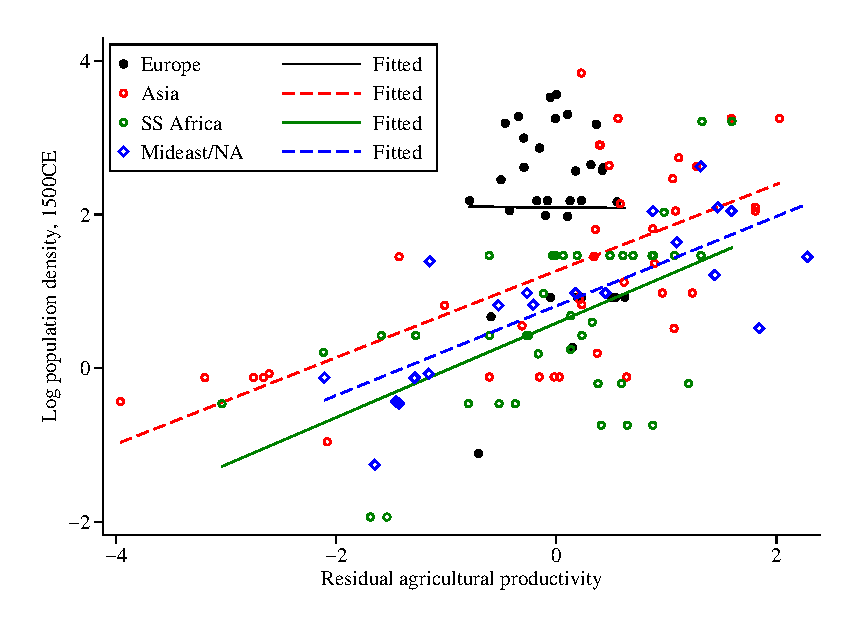
\includegraphics[width=1.0\textwidth]{fig_ag_regions.eps}
\end{center}
\vspace{-.5cm}\singlespacing {\footnotesize \textbf{Notes}: The figure replicates, by region, the regression from \citet{ashraf2010dynamics}, Table 2, column (4). We plot raw  population density in 1500CE against the residual variation in agricultural productivity, after controlling for (log) years since the Neolithic transition, (log) absolute latitude, the mean distance to a coast or river, and the percent of land less than 100 km from a coast or river. Agricultural productivity, from \citet{ashraf2010dynamics}, is the first principal component of the percent of arable land and a measure of cultivation suitability from \citet{ramankutty2002}. See appendix for lists of exact countries included in each region.
}
\end{figure}

\clearpage

\begin{figure}[!htb]
\begin{center}
\caption{Density Plot of Caloric Yield ($A_{isc}$), by Region}
\label{FIG_dens_csi}
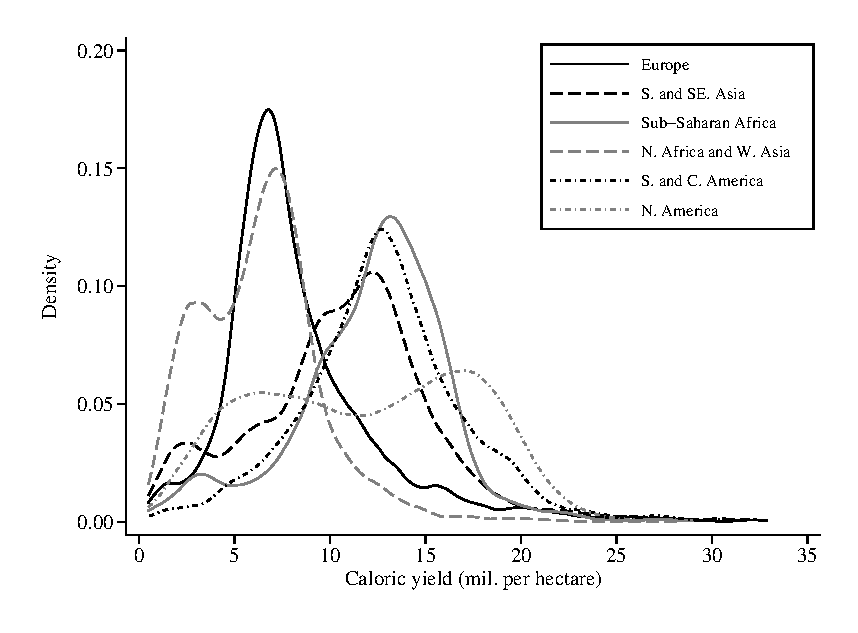
\includegraphics[width=1.0\textwidth]{fig_dens_csi.eps}
\end{center}
\vspace{-.5cm}\singlespacing {\footnotesize \textbf{Notes}: Kernel density plot, Epanechnikov kernel, of the caloric yield, $A_{isc}$, at the district level, calculated by the authors using data from \citet{galorozak2016}. See text for details. This measure sums the maximum calories available per grid cell within a district, then divides by total area of the district. See appendix for lists of exact countries included in each region.
}
\end{figure}

\clearpage

%\begin{figure}[!htb]
%\begin{center}
%\caption{Density Plot of Log Rural Density ($L_{Aisc}/X_{isc}$), by Region, 2000CE}
%\label{FIG_dens_rurd}
%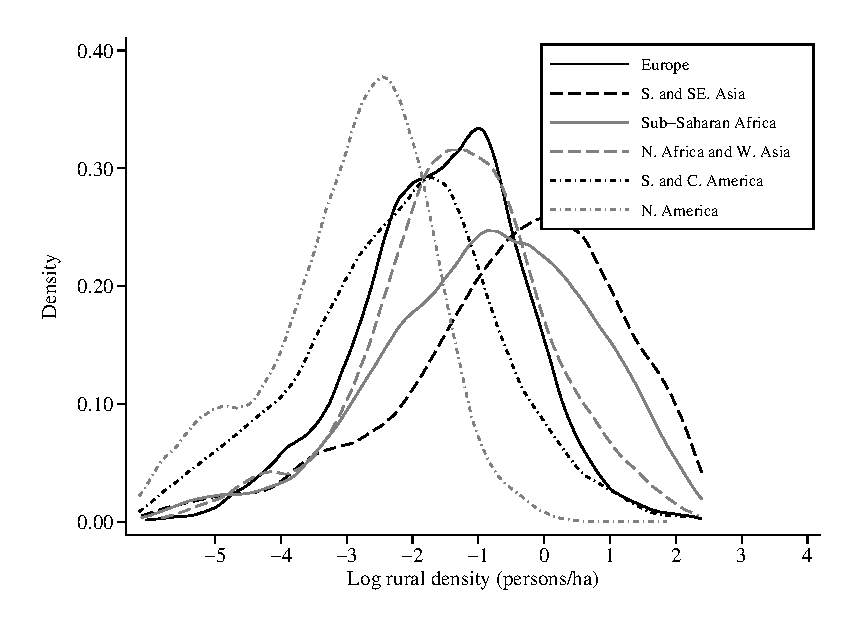
\includegraphics[width=1.0\textwidth]{fig_dens_rurd.eps}
%\end{center}
%\vspace{-.5cm}\singlespacing {\footnotesize \textbf{Notes}:Kernel density plot, Epanechnikov kernel, of the (log) rural density, $L_{Aisc}/X_{isc}$, at the district level, calculated by the authors using data from \citet{hyde31} for rural population. See text for details. See appendix for lists of exact countries included in each region.
%}
%\end{figure}

\clearpage

\begin{figure}[!htb]
\begin{center}
\caption{Province-Level Estimates of $\beta$, and Medians, by Sub-region, 2000CE}
\label{FIG_beta_province}
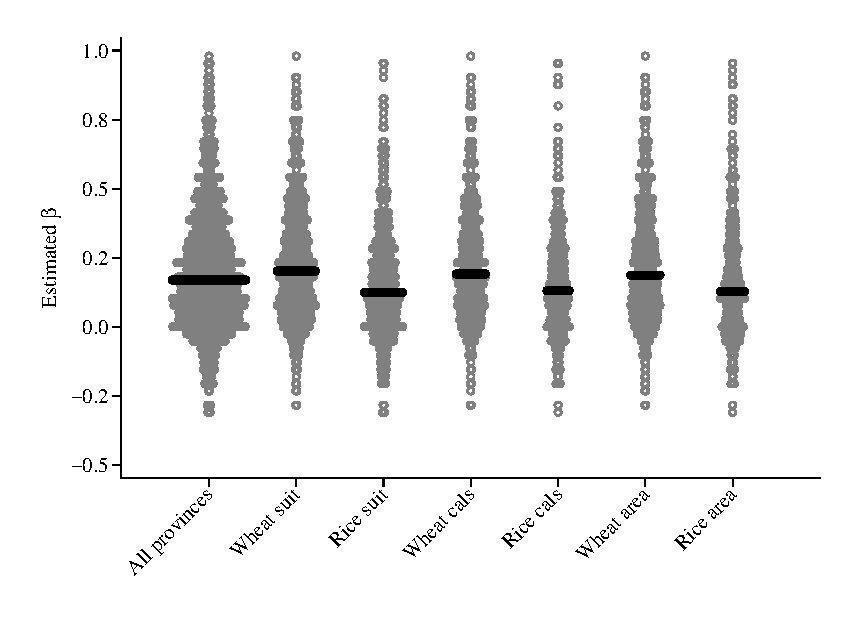
\includegraphics[width=1.0\textwidth]{fig_beta_province.eps}
\end{center}
\vspace{-.5cm}\singlespacing {\footnotesize \textbf{Notes}: The figure shows the distribution of $\hat{\beta}$ values within each sub-region. Within a sub-region, province level estimates are grouped into (up to) 50 bins, and each province is plotted in gray using the middle value of that bin, with the width of each bin indicating the number of provinces contained within it. The black lines indicate the median estimate value of $\beta$ within the entire sub-region. Prior to plotting, values of $\beta$ were trimmed at the 1st and 99th percentiles of the entire sample.
}
\end{figure}


\clearpage


\begin{figure}[!htb]
\begin{center}
\caption{Caloric Yield and Rural Density, by Major Crop, 2000CE}
\label{FIG_beta_crop}
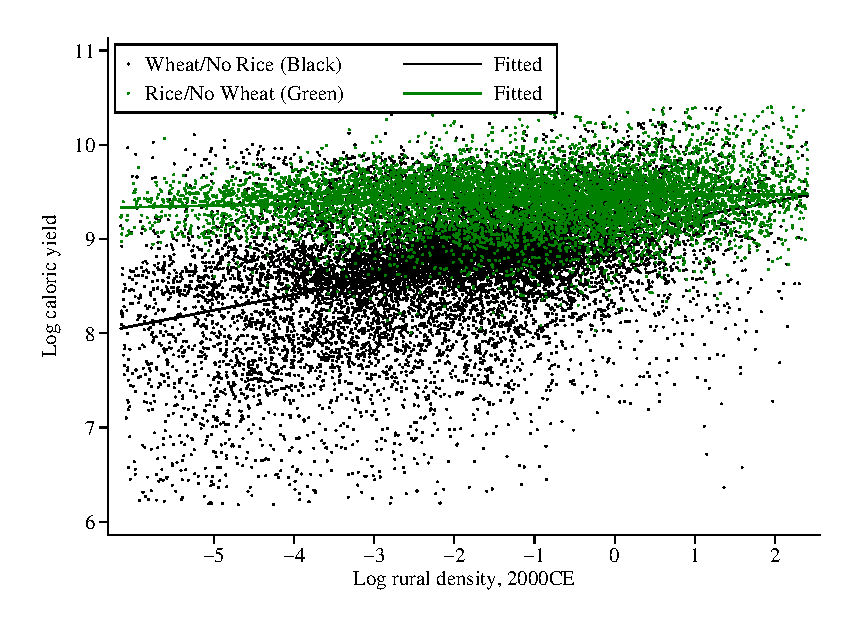
\includegraphics[width=1.0\textwidth]{fig_beta_crop.eps}
\end{center}
\vspace{-.5cm}\singlespacing {\footnotesize \textbf{Notes}: This figures shows the raw correlation of (log) caloric yield and (log) rural density for districts that are (a) suitable for wheat, but not for rice, and (b) suitable for rice but not for wheat. Rural population is from HYDE database \citep{hyde31}, and caloric yield is the author's calculations based on the data from \citet{galorozak2016}. The linear fits are from bivariate OLS regressions, without country fixed effects included.
}
\end{figure}


\clearpage

\begin{figure}[!htp]
\begin{center}
	\subfigure{
	  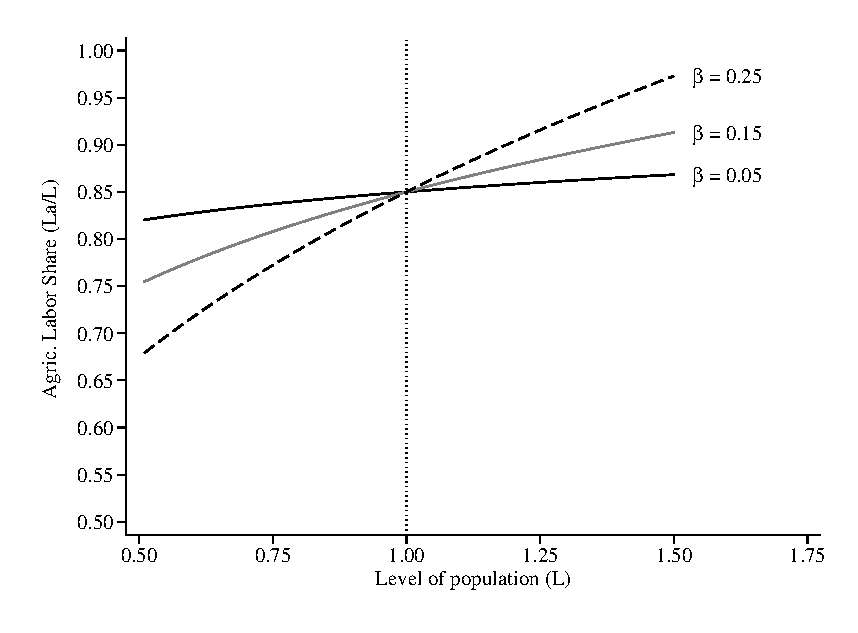
\includegraphics[width=3in]{fig_sim_L_LaL.eps}
	}
	\subfigure{
	  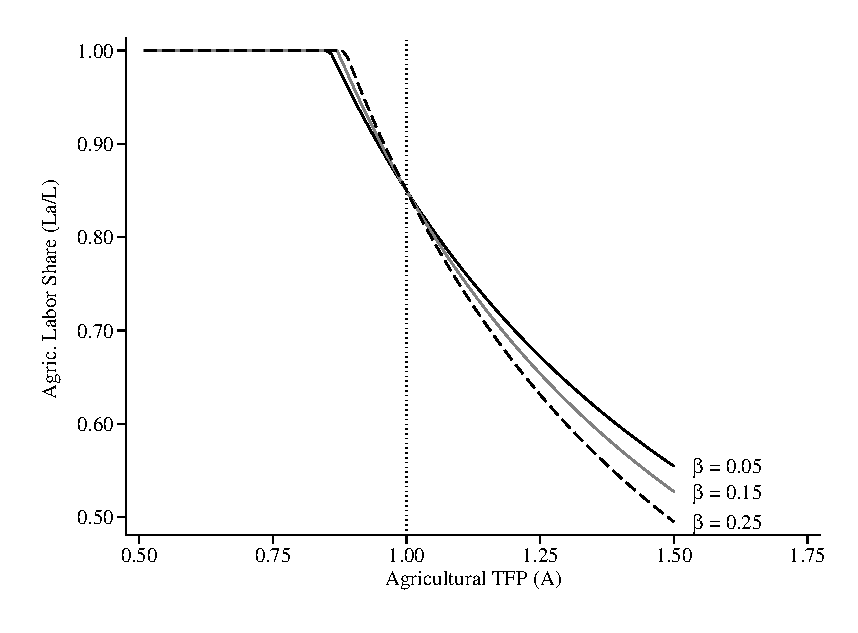
\includegraphics[width=3in]{fig_sim_A_LaL.eps}
	}
	\subfigure{
	  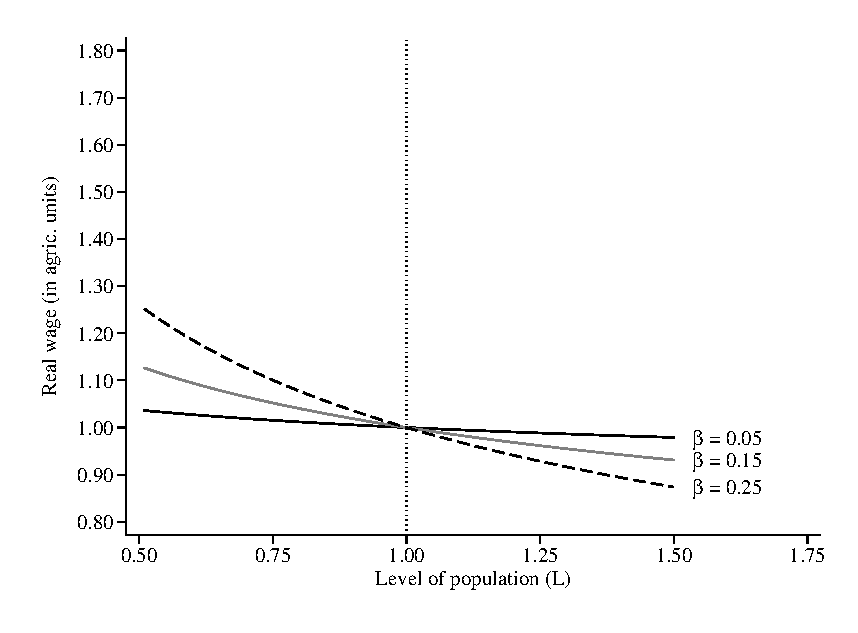
\includegraphics[width=3in]{fig_sim_L_w.eps}
	}	
	\subfigure{
	  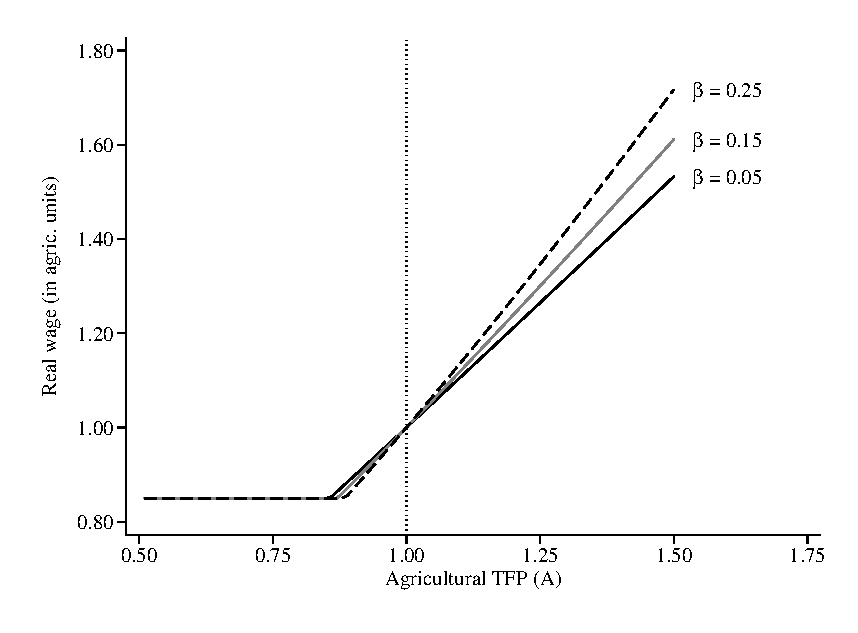
\includegraphics[width=3in]{fig_sim_A_w.eps}
	}
\caption{The Effect of Shocks on Outcomes, by size of $\beta$} \label{FIG_sim_L}
\end{center}
\singlespacing {\footnotesize  \textbf{Notes}: The sub-figures show the effects of either changes in population (left) or agricultural TFP (right) on the share of labor in agriculture (top) or the real wage (bottom). Within each sub-figure, the effects are shown for three different simulations that differ only in the tightness of their land constraint, $\beta$. Each simulation is given a value of agricultural consumption per person, $c_A$, such that with a population of $L = 1$ and agricultural TFP of $A = 1$, the labor share in agriculture is $L_A/L = 0.85$. See text for details on the equations used to calculate the response of real wages and labor share in agriculture to changes in $L$ and $A$.
}
\end{figure}


\clearpage

\begin{table}[!htb]
\begin{center}
\caption{Population Density and Land Productivity, by Region, 1500CE}
\label{TAB_ag_regions}
{\small
\begin{tabularx}{\textwidth}{lXXXXXX}
\midrule
\multicolumn{7}{l}{Dependent Variable: Log population density:} \\
 & \multicolumn{6}{c}{Region:} \\ \cmidrule{2-7}
 &        &      &         & Sub-      & North     & \\
 &        &      &         & Saharan   & Africa \& & \\
 & All & Europe  & Asia    & Africa    & Mideast & Americas \\
 & (1) & (2) & (3) & (4) & (5) & (6) \\
\midrule
Log Land Productivity&       0.533&      -0.013&       0.558&       0.615&       0.583&       0.324\\
                    &     (0.059)&     (0.427)&     (0.062)&     (0.116)&     (0.070)&     (0.308)\\
\midrule
Observations        &         147&          33&          40&          39&          21&          25\\
Adjusted R-square   &        0.67&        0.39&        0.65&        0.71&        0.80&        0.46\\

\midrule
\end{tabularx}
}
\end{center}
\vspace{-.5cm}\singlespacing {\footnotesize \textbf{Notes}: Standard errors are robust. Regression (1) includes continent fixed effects for Europe, Asia, and Africa; the Americas is the excluded category, and the North Africa/Mid-east category overlaps with Asia and Africa. See appendix for lists of exact countries included in each region. All regressions includes controls (log) years since the Neolithic transition, (log) absolute latitude, the mean distance to a coast or river, and the percent of land less than 100 km from a coast or river. The data is drawn directly from \citet{ashraf2010dynamics}, and column (1) replicates their result.
}
\end{table}

\clearpage

\begin{table}[!htb]
\begin{center}
\caption{Summary Statistics for District Level Data, 2000CE}
\label{TAB_summ}
{\small
\begin{tabularx}{\textwidth}{lXXXXXXX}
\midrule
 &      &            & \multicolumn{5}{c}{Percentiles:} \\ \cmidrule{4-8}
 & Mean & SD  & 10th    & 25th    & 50th & 75th & 90th \\
\midrule
Labor/land (persons/ha) &     0.73&     1.17&     0.04&     0.12&     0.32&     0.77&     1.86\\
Caloric yield (mil cals/ha) &    10.85&     4.89&     4.98&     7.17&    10.65&    13.86&    17.03\\
Log light density &    -2.82&     2.93&    -6.14&    -3.83&    -2.51&    -0.89&     0.35\\

\midrule
\end{tabularx}
}
\end{center}
\vspace{-.5cm}\singlespacing {\footnotesize \textbf{Notes}: A total of 32,862 observations for each variable (these come from 2,471 provinces in 154 countries). Caloric yield, $A_{isc}$ calculated by the authors using data from \citet{galorozak2016}. Rural density, $L_{Aisc}/X_{isc}$ calculated by the authors using data from \citet{hyde31} for rural population. Both caloric yield and rural density were trimmed at the 99th and 1st percentiles of their raw data prior to calculating the summary statistics in this table. Urbanization rate taken from \citet{hyde31}. Log mean light density derived from the Global Radiance Calibrated Nightime Lights data provided by NOAA/NGDC, as in \citet{hssw2016}. 
}
\end{table}


\clearpage
\begin{table}[!htb]
\begin{center}
\caption{Estimates of Malthusian Tightness, $\beta$, by Region, 2000CE}
\label{TAB_beta_region}
{\small
\begin{tabularx}{\textwidth}{lXXXXXX}
\midrule
\multicolumn{7}{l}{Dependent Variable: Log caloric yield ($A_{isc}$)} \\
 & \multicolumn{6}{c}{Region:} \\ \cmidrule{2-7}
 &        & East \& & Sub-        & North     & South \&  &  \\
 &        & South   & Saharan     & Africa \& & Central   & U.S. and \\
 & Europe & Asia    & Africa      & West Asia & America   & Canada \\
 & (1) & (2) & (3) & (4) & (5) & (6) \\
\midrule
Log rural density   &       0.279&       0.157&       0.104&       0.213&       0.119&       0.203\\
                    &     (0.027)&     (0.017)&     (0.014)&     (0.035)&     (0.017)&     (0.044)\\
\midrule
p-value $\beta=0$   &       0.000&       0.000&       0.000&       0.000&       0.000&       0.000\\
p-value $\beta=\beta^{Eur}$&           .&       0.000&       0.000&       0.137&       0.000&       0.142\\
Countries           &          34&          24&          43&          18&          25&           2\\
Observations        &        7514&        6761&        3210&        2762&        9131&        2782\\
Adjusted R-square   &        0.30&        0.24&        0.26&        0.28&        0.18&        0.28\\

\midrule
\end{tabularx}
}
\end{center}
\vspace{-.5cm}\singlespacing {\footnotesize \textbf{Notes}: Conley standard errors, adjusted for spatial auto-correlation with a cutoff distance of 500km, are shown in parentheses. All regressions include province fixed effects, a constant, and controls for the district urbanization rate and log density of district nighttime lights. See appendix for lists of exact countries included in each region. The coefficient estimate on rural population density indicates the value of $\beta$, see equation (\ref{EQ_regress}). Rural population is from HYDE database \citep{hyde31}, and caloric yield is the author's calculations based on the data from \citet{galorozak2016}. The p-value is from a hypothesis test that the estimated $\beta$ is equal to that estimated for Europe, $\beta^{Eur}$, and is obtained from an interaction term in a separate regression including both Europe and the given region, see equation (\ref{EQ_interaction}) and the text for details.
}
\end{table}


\clearpage
\begin{table}[!htb]
\begin{center}
\caption{Estimates of Malthusian Tightness, $\beta$, by Sub-regions, 2000CE}
\label{TAB_beta_subregion}
{\small
\begin{tabularx}{\textwidth}{lXXXXX}
\midrule
\multicolumn{6}{l}{Dependent Variable in both panels: Log caloric yield ($A_{isc}$)} \\ \\
\\
Panel A & \multicolumn{5}{c}{Sub-Region:} \\ \cmidrule{2-6}
 &          &         &             &  \multicolumn{2}{c}{Excl. China, Japan, Korea} \\ \cmidrule(lr){5-6}
 & North \& &         &              & South \&  & Central \&             \\
 & Western  & Eastern & Southern     & Southeast & West        \\
 & Europe   & Europe  & Europe       & Asia      & Asia      \\
 & (1) & (2) & (3) & (4) & (5) \\
\midrule
Log rural density   &       0.264&       0.292&       0.271&       0.148&       0.184\\
                    &     (0.040)&     (0.032)&     (0.043)&     (0.027)&     (0.028)\\
\midrule
p-value $\beta=0$   &       0.000&       0.000&       0.000&       0.000&       0.000\\
p-value $\beta=\beta^{NWEur}$&           .&       0.569&       0.884&       0.016&       0.099\\
Countries           &          16&           9&           9&          13&          18\\
Observations        &        1628&        4772&        1114&        3921&        2762\\
Adjusted R-square   &        0.21&        0.31&        0.26&        0.16&        0.18\\

\midrule
\\
Panel B & \multicolumn{5}{c}{Sub-Region:} \\ \cmidrule{2-6}
 &           &   &           &          &             \\
 & Temperate & Tropical  & Tropical & South    & North    \\
 & Americas  & Americas  & Africa   & Africa   & Africa     \\
\midrule
Log rural density   &       0.187&       0.119&       0.100&       0.130&       0.282\\
                    &     (0.039)&     (0.018)&     (0.013)&     (0.071)&     (0.010)\\
\midrule
p-value $\beta=0$   &       0.000&       0.000&       0.000&       0.066&       0.000\\
p-value $\beta=\beta^{NWEur}$&       0.170&       0.001&       0.000&       0.099&       0.654\\
Countries           &           5&          22&          39&           4&           5\\
Observations        &        3183&        8730&        3032&         178&        1147\\
Adjusted R-square   &        0.18&        0.10&        0.14&        0.19&        0.24\\

\midrule
\end{tabularx}
}
\end{center}
\vspace{-.5cm}\singlespacing {\footnotesize \textbf{Notes}: Conley standard errors, adjusted for spatial auto-correlation with a cutoff distance of 500km, are shown in parentheses. All regressions include province fixed effects, a constant, and controls for the district urbanization rate and log density of district nighttime lights. See appendix for lists of exact countries included in each region. The coefficient estimate on rural population density indicates the value of $\beta$, see equation (\ref{EQ_regress}). Rural population is from HYDE database \citep{hyde31}, and caloric yield is the author's calculations based on the data from \citet{galorozak2016}. The p-value is from a hypothesis test that the estimated $\beta$ is equal to that estimated for Northwest Europe, $\beta^{NWEur}$, and is obtained from an interaction term in a separate regression including both Northwest Europe and the given region, see equation (\ref{EQ_interaction}) and the text for details.
}
\end{table}

\clearpage
\begin{table}[!htb]
\begin{center}
\caption{Estimates of Malthusian Tightness, $\beta$, China, Japan, and Korea, 2000CE}
\label{TAB_beta_china}
{\small
\begin{tabularx}{\textwidth}{lXXXXX}
\midrule
\multicolumn{4}{l}{Dependent Variable: Log caloric yield ($A_{isc}$)} \\
 & All& Temperate & Sub-Tropical & & North \& \\
 & China & China  & China & Japan & South Korea  \\
 & (1) & (2) & (3) & (4) & (5) \\
\midrule
Residuals           &       0.414&       0.518&       0.107&       0.155&       0.190\\
                    &     (0.089)&     (0.060)&     (0.021)&     (0.003)&     (0.060)\\
\midrule
p-value $\beta=0$   &       0.000&       0.000&       0.000&       0.000&       0.002\\
p-value $\beta=\beta^{Temp}$&            &            &       0.000&            &            \\
Observations        &         266&         130&         136&        1039&         311\\
Adjusted R-square   &        0.56&        0.70&        0.13&        0.23&        0.23\\

\midrule
\end{tabularx}
}
\end{center}
\vspace{-.5cm}\singlespacing {\footnotesize \textbf{Notes}: Conley standard errors, adjusted for spatial auto-correlation with a cutoff distance of 500km, are shown in parentheses. All regressions include province fixed effects, a constant, and controls for the district urbanization rate and log density of district nighttime lights. See appendix for lists of exact countries included in each region. The coefficient estimate on rural population density indicates the value of $\beta$, see equation (\ref{EQ_regress}). Rural population is from HYDE database \citep{hyde31}, and caloric yield is the author's calculations based on the data from \citet{galorozak2016}. The p-value is from a hypothesis test that the estimated $\beta$ is equal to that estimated for temperate China, $\beta^{Temp}$, and is obtained from an interaction term in a separate regression including both temperate and sub-tropical China, see equation (\ref{EQ_interaction}) and the text for details.
}
\end{table}

\clearpage

\begin{table}[!htb]
\begin{center}
\caption{Summary Statistics for Individual Province $\beta$ Estimates, by Sub-region, 2000CE}
\label{TAB_beta_province}
{\small
\begin{tabularx}{\textwidth}{lrXrXrXrXrXrXrXr}
\midrule
           &       &&      &&     && \multicolumn{9}{c}{Percentiles:} \\ \cmidrule{8-16}
Sub-region & Prov. && Mean && SD  && 10th    && 25th    && 50th && 75th && 90th \\
\midrule
All provinces &    1,183&     0.21&     0.23&    -0.02&     0.05&     0.18&     0.33&     0.49\\ \\
Wheat Suitable &      619&     0.23&     0.23&    -0.00&     0.08&     0.21&     0.36&     0.50\\
Rice Suitable &      469&     0.17&     0.24&    -0.04&     0.03&     0.15&     0.28&     0.43\\
Wheat cals>33\% &      457&     0.23&     0.22&    -0.00&     0.08&     0.21&     0.36&     0.50\\
Rice cals>33\% &      307&     0.18&     0.21&    -0.04&     0.03&     0.15&     0.29&     0.41\\
Wheat area>50\% &      485&     0.22&     0.23&    -0.01&     0.07&     0.20&     0.36&     0.53\\
Rice area>50\% &      297&     0.18&     0.23&    -0.04&     0.03&     0.14&     0.29&     0.47\\ \\
Northwest Europe &        79&     0.26&     0.31&     0.00&     0.08&     0.22&     0.46&     0.62\\
Eastern Europe &       173&     0.24&     0.20&     0.01&     0.09&     0.23&     0.38&     0.50\\
Southern Europe &        60&     0.27&     0.17&     0.08&     0.16&     0.25&     0.37&     0.50\\
South and S. East Asia &       248&     0.20&     0.23&    -0.03&     0.04&     0.16&     0.31&     0.49\\
Central and West. Asia &       163&     0.20&     0.20&    -0.02&     0.06&     0.16&     0.33&     0.45\\
Temperate Americas &        87&     0.14&     0.25&    -0.13&     0.02&     0.10&     0.26&     0.40\\
Tropical Americas &       195&     0.18&     0.26&    -0.02&     0.06&     0.17&     0.28&     0.39\\
Tropical Africa &       118&     0.16&     0.24&    -0.09&    -0.01&     0.09&     0.25&     0.51\\
Southern Africa &        11&     0.15&     0.21&    -0.11&    -0.05&     0.17&     0.33&     0.34\\
Northern Africa &        49&     0.32&     0.20&     0.06&     0.22&     0.31&     0.42&     0.66\\

\midrule
\end{tabularx}
}
\end{center}
\vspace{-.5cm}\singlespacing {\footnotesize \textbf{Notes}: The value of $\beta$ was estimated separately for each province, as described in the text. For each sub-region, the table shows the summary statistics of $\beta$ for provinces that are located in that sub-region. Provinces were only included if they have 6 or more districts within them.
}
\end{table}


\clearpage


\begin{table}[!htb]
\begin{center}
\caption{Estimates of Malthusian Tightness, $\beta$, by Crop Suitability, 2000CE}
\label{TAB_beta_crops}
{\footnotesize
\begin{tabularx}{\textwidth}{lXXXXXX}
\midrule
\multicolumn{7}{l}{Dependent Variable in all panels: Log caloric yield ($A_{isc}$)} \\ \\
\multicolumn{7}{l}{Panel A: Wheat and rice} \\
 & \multicolumn{6}{c}{Inclusion by crop suitability:} \\ \cmidrule(lr){2-7}
 & \multicolumn{4}{c}{Entire world:} & \multicolumn{2}{c}{Ex. Americas:}\\ \cmidrule(lr){2-5} \cmidrule(lr){6-7} 
 & Wheat$>$0& Wheat=0 &         &        & Wheat$>$0   & Wheat=0   \\
 & Rice=0 & Rice$>$0  & Wheat$>$0 & Rice$>$0 & Rice=0    & Rice$>$0   \\
 & (1) & (2) & (3) & (4) & (5) & (6) \\
\midrule
rurd_reg            &       0.227&       0.138\\
                    &     (0.024)&     (0.021)\\
\midrule
p-value $\beta=0$   &       0.000&       0.000\\
p-value $\beta=\beta^{Wheat}$&            &    .0049448\\
Countries           &         106&          74\\
Observations        &    12627.00&    20423.00\\
Adjusted R-square   &        0.21&        0.19\\

\midrule
\\
\multicolumn{7}{l}{Panel B: Tropical crops} \\
                   & \multicolumn{6}{c}{Inclusion is wheat suitability = 0, but:} \\ \cmidrule(lr){2-7}
                   &            &              &          &   Pearl       &  Sweet      & \\
& Cassava$>$0 & Cowpeas$>$0  & Maize$>$0 & Millet$>$0 & Potato$>$0 & Yams$>$0   \\
\midrule
Log rural density   &       0.140&       0.144&       0.143&       0.154&       0.144&       0.140\\
                    &     (0.021)&     (0.020)&     (0.020)&     (0.019)&     (0.020)&     (0.020)\\
\midrule
p-value $\beta=0$   &       0.000&       0.000&       0.000&       0.000&       0.000&       0.000\\
Countries           &          74&          80&          78&          72&          77&          78\\
Observations        &        8052&        8312&        8377&        6590&        8354&        8269\\
Adjusted R-square   &        0.13&        0.13&        0.13&        0.13&        0.13&        0.12\\

\midrule
\\
\multicolumn{7}{l}{Panel C: Temperate crops} \\
                   & \multicolumn{6}{c}{Inclusion is rice suitability = 0, but:} \\ \cmidrule(lr){2-7}
                   &            & Buck-        &          &          &         & White \\
                   & Barley$>$0 & wheat$>$0  & Oats$>$0 & Flax$>$0 & Rye$>$0 & Potato$>$0   \\
\midrule
Log rural density   &       0.227&       0.228&       0.234&       0.228&       0.235&       0.227\\
                    &     (0.024)&     (0.025)&     (0.025)&     (0.025)&     (0.025)&     (0.023)\\
\midrule
p-value $\beta=0$   &       0.000&       0.000&       0.000&       0.000&       0.000&       0.000\\
Countries           &         106&          76&          72&          74&          72&         105\\
Observations        &       12627&       11162&       11089&       11035&       11106&       12494\\
Adjusted R-square   &        0.21&        0.23&        0.23&        0.23&        0.23&        0.22\\

\midrule
\end{tabularx}
}
\end{center}
\vspace{-.5cm}\singlespacing {\footnotesize \textbf{Notes}: Conley standard errors, adjusted for spatial auto-correlation with a cutoff distance of 500km, are shown in parentheses. All regressions include province fixed effects, a constant, and controls for the district urbanization rate and log density of district nighttime lights. The coefficient estimate on rural population density indicates the value of $\beta$, see equation (\ref{EQ_regress}). Rural population is from HYDE database \citep{hyde31}, and caloric yield is the author's calculations based on the data from \citet{galorozak2016}. Inclusion of sub-national units in the regression is based on crop suitability indices from \citet{gaez}, which range from 0 to 100, and are calculated by the author's for each sub-national unit. See text for details.
}
\end{table}


\begin{table}[!htb]
\begin{center}
\caption{Estimates of Malthusian Tightness, $\beta$, by K{\"o}ppen-Geiger Zone, 2000CE}
\label{TAB_beta_kg}
{\footnotesize
\begin{tabularx}{\textwidth}{lXXXXXX}
\midrule
\multicolumn{7}{l}{Dependent Variable in all panels: Log caloric yield ($A_{isc}$)} \\ \\
\multicolumn{7}{l}{Panel A: Climate Zones} \\
 & Equatorial & Arid  & Temperate & Snow &     &   \\
 & (1) & (2) & (3) & (4) &  & \\
\midrule
Log rural density   &       0.118&       0.154&       0.171&       0.237\\
                    &     (0.018)&     (0.034)&     (0.024)&     (0.031)\\
\midrule
p-value $\beta=0$   &       0.000&       0.000&       0.000&       0.000\\
Countries           &          81&          57&          94&          43\\
Observations        &       10752&        2675&       13019&        6058\\
Adjusted R-square   &        0.11&        0.09&        0.17&        0.27\\

\midrule
\\
\multicolumn{7}{l}{Panel B: Precipitation Zones} \\
& Fully     & Dry         & Dry        &              &            & \\
& Humid & Summer  & Winter & Monsoons & Desert & Steppe   \\
 & (1) & (2) & (3) & (4) & (5) & (6) \\
\midrule
Log rural density   &       0.187&       0.183&       0.127&       0.135&       0.109&       0.116\\
                    &     (0.033)&     (0.030)&     (0.021)&     (0.029)&     (0.039)&     (0.031)\\
\midrule
p-value $\beta=0$   &       0.000&       0.000&       0.000&       0.000&       0.005&       0.000\\
Countries           &          99&          46&          75&          43&          34&          55\\
Observations        &       16371&        3067&        8683&        1729&         390&        2270\\
Adjusted R-square   &        0.19&        0.19&        0.12&        0.12&        0.04&        0.06\\

\midrule
\\
\multicolumn{7}{l}{Panel C: Temperature Zones} \\
    & Hot        & Warm        & Cool       & Hot      & Cold     &  \\
    & Summer & Summer  & Summer & Arid & Arid &   \\
 & (1) & (2) & (3) & (4) & (5) &  \\    
\midrule
Log rural density   &       0.141&       0.227&       0.254&       0.135&       0.142\\
                    &     (0.020)&     (0.034)&     (0.047)&     (0.032)&     (0.045)\\
\midrule
p-value $\beta=0$   &       0.000&       0.000&       0.000&       0.000&       0.002\\
Countries           &          61&          86&          26&          45&          26\\
Observations        &        8749&        9751&         487&        1594&        1065\\
Adjusted R-square   &        0.15&        0.25&        0.13&        0.07&        0.09\\

\midrule
\end{tabularx}
}
\end{center}
\vspace{-.5cm}\singlespacing {\footnotesize \textbf{Notes}: Conley standard errors, adjusted for spatial auto-correlation with a cutoff distance of 500km, are shown in parentheses. All regressions include province fixed effects, a constant, and controls for the district urbanization rate and log density of district nighttime lights. The coefficient estimate on rural population density indicates the value of $\beta$, see equation (\ref{EQ_regress}). Rural population is from HYDE database \citep{hyde31}, and caloric yield is the author's calculations based on the data from \citet{galorozak2016}. Inclusion of districts is based on whether they have more than 50\% of their land area in the given K{\"o}ppen-Geiger zone. See text for details.
}
\end{table}

\end{document}